\documentclass[12pt,letterpaper,oneside,final]{book}		
\usepackage[lmargin=3.0cm,rmargin=2.5cm,tmargin=2.5cm,bmargin=2.5cm]{geometry}
\usepackage[table]{xcolor}
\usepackage{setspace}
\usepackage{tabulary}
\usepackage{mfirstuc}
\usepackage{graphicx}
\usepackage{multicol}
\usepackage{caption}
\usepackage{float}
\usepackage{wrapfig}
\usepackage{lipsum}
\usepackage{ifpdf}
\usepackage[utf8]{inputenc}
\usepackage[T1]{fontenc}
\usepackage[]{times}
\usepackage[spanish]{babel}
\usepackage[nottoc]{tocbibind}
\usepackage{hyperref}
\usepackage{amsmath,amssymb}
\usepackage{array}
\usepackage{afterpage}
\usepackage{subcaption}
\usepackage{makeidx}
\usepackage{color}
\usepackage{adjustbox}
% \usepackage{refcheck} % checks for unreferenced labels
\usepackage{datetime}
\usepackage{acro}
\usepackage{mfirstuc}% provides \capitalisewords
\usepackage{parskip}
\usepackage{fancyhdr}

\acsetup{list-long-format=\capitalisewords}

\fancypagestyle{newstyle}{
\fancyhf{} % clear all header and footer fields
\fancyhead[l]{} % except the center
\fancyfoot[R]{\thepage} % except the center
\renewcommand{\headrulewidth}{0pt}
\renewcommand{\footrulewidth}{0pt}}

\pagestyle{newstyle}

% \norefnames % no margin ref names
% \nocitenames % no margin cite names

\makeindex
% \usepackage{showframe}
\ifpdf
  \usepackage{epstopdf}
\fi

\onehalfspacing
\setlength{\parindent}{4em}

\renewcommand\floatpagefraction{.9}
\renewcommand\topfraction{.9}
\renewcommand\bottomfraction{.9}
\renewcommand\textfraction{.1}
\addto\captionsspanish{%
  \renewcommand{\tablename}%
    {Tabla}%
}

\setcounter{totalnumber}{50}
\setcounter{topnumber}{50}
\setcounter{bottomnumber}{50}

% Different font in captions
\newcommand{\captionfonts}{\small}

\makeatletter  % Allow the use of @ in command names
\long\def\@makecaption#1#2{%
  \vskip\abovecaptionskip
  \sbox\@tempboxa{{\captionfonts #1: #2}}%
  \ifdim \wd\@tempboxa >\hsize
    {\captionfonts #1: #2\par}
  \else
    \hbox to\hsize{\hfil\box\@tempboxa\hfil}%
  \fi
  \vskip\belowcaptionskip}
\makeatother   % Cancel the effect of \makeatletter

\hypersetup{
    colorlinks,
    citecolor=black,
    filecolor=black,
    linkcolor=black,
    urlcolor=black
}

\newcommand\blankpage{%
    \null
    \thispagestyle{empty}%
    \addtocounter{page}{-1}%
    \newpage
}

\newcommand{\quotemarks}[1]{``#1''} 

\newdateformat{monthyeardate}{%
  \monthname[\THEMONTH] del \THEYEAR}

\DeclareAcronym{BRDF}{
  short = BRDF ,
  long  = función de distribución de reflectancia bidireccional
}
\DeclareAcronym{BSSRDF}{
  short = BSSRDF ,
  long  = función de distribución de reflectancia y transluminiscencia bidireccional
}
\DeclareAcronym{NDF}{
  short = NDF ,
  long  = función de distribución normal
}
\DeclareAcronym{CLPV}{
  short = CLPV ,
  long  = volúmenes de propagación de luz en cascada
}
\DeclareAcronym{LPV}{
  short = LPV,
  long  = volumen de propagación de luz
}
\DeclareAcronym{GV}{
  short = GV ,
  long  = volumen de geometría
}
\DeclareAcronym{RSM}{
  short = RSM ,
  long  = mapas de sombras reflexivo
}
\DeclareAcronym{VPL}{
  short = VPL ,
  long  = luz puntual virtual
}
\DeclareAcronym{GBuffer}{
  short = G-Buffer ,
  long  = buffer de geometría
}
\DeclareAcronym{VCT}{
  short = VCT,
  long  = trazado vóxeles con conos
}
\DeclareAcronym{GPU}{
  short = GPU,
  long  = unidad de procesamiento grafico
}
\DeclareAcronym{GPGPU}{
  short = GPGPU,
  long  = cómputo de propósito general en la unidad de procesamiento grafico
}



\setcounter{tocdepth}{3}
\setcounter{secnumdepth}{3}

\begin{document}
  \frontmatter
  % portada
  \label{ch:portada}
\thispagestyle{empty}

\begin{figure}[t]
    \centering
    \includegraphics[height=0.15\textwidth]{media/logoucv.eps}
\end{figure}

\begin{center}
	Universidad Central de Venezuela\\
	Facultad de Ciencias\\
	Escuela de Computaci\'on\\
	Centro de Computaci\'on Gr\'afica\\
\end{center}
				
\vspace{2.5cm}

\begin{center}
	\large{\textbf{Trazado de Conos para el Cálculo de Iluminación\\ Global empleando Sombreado de Vóxeles}}
\end{center}
				
\vspace{2.5cm}

\begin{center}
    Trabajo Especial de Grado presentado ante la Ilustre\\
    Universidad Central de Venezuela \\
    por el Br. José Gabriel Villegas Guedez\\
    para optar al título de Licenciado en Computación.
\end{center}

\vspace{2.5cm}				
				
\begin{center}
	Tutor:\\
	Prof. Esmitt Ramírez
\end{center}
				
\vspace{\fill}

\begin{center}
	Caracas, \monthyeardate\today
\end{center}

\newpage
\includepdf{Acta.pdf}			
  % resumen
  \section*{Resumen}
La iluminación de escenas es fundamental para la generación de imágenes de alta calidad, esta provee inmersión, sensación de profundidad y realismo. La producción de iluminación realista comprende, entre muchas otras cosas, la inclusión de iluminación indirecta para la composición de iluminación global.

Existen varios algoritmos para el cálculo de la iluminación global de forma analítica, sin embargo el costo computacional de estos es alto y dependiente de la complejidad de la escena. Esto hace estas soluciones poco flexibles o simplemente inadecuadas para aplicaciones en tiempo real, altamente interactivas o de considerable complejidad geométrica. 

Con el incremento de la capacidad de cómputo en las unidades de procesamiento gráfico modernas también ha aumentado el interés por la inclusión de fenómenos de iluminación global en aplicaciones en tiempo real. De esto han surgido una variada cantidad de aproximaciones explotando características del hardware de procesamiento gráfico y los recursos disponibles en el pipeline de renderizado. Estos algoritmos mantienen cierto grado de coherencia o convergen con la solución analítica al problema de iluminación global. 

Este trabajo tiene como enfoque principal el renderizado de iluminación global en tiempo real, por esto se realiza una investigación de estos algoritmos y se presenta el desarrollo de una aplicación con iluminación global utilizando trazado de vóxeles y conos.
\paragraph{Palabras Clave:}
Iluminación global, vóxeles, trazado de conos, iluminación indirecta, unidad de cómputo gráfico, renderizado en tiempo real.

\newpage
\section*{Agradecimientos}

Al profesor Esmitt Ramírez, por su apoyo y dirección, sin el cual este trabajo de investigación se hubiese llevado a cabo.

A mi mamá, Marina Villegas, por su apoyo y soporte incondicional en todos los aspectos de mi vida y por ser mi mejor amiga. 

A mi hermano menor Daniel De La Cruz, por su colaboración y ayuda para hacer este trabajo posible e inspirarme a ser un buen ejemplo para él.

A todos mis amigos por estar siempre atentos a este trabajo y su progreso el cual me mantuvo enfocado durante la realización de este trabajo. Y además por ser los causantes de múltiples distracciones cuando las necesitaba y no necesitaba.
  % Tabla de contenido, indice
  \tableofcontents
  % contenido
  % \printacronyms[include-classes=abbrev,name=Abreviaturas]
  \afterpage{\blankpage} % pagina vacia despues del indice
  % introducction
  \addcontentsline{toc}{chapter}{Introducción}
\chapter*{Introducción}
\label{ch:intro}
  % objetivos generales y specificos
  \include{introduction/goals}
  % after introduction main matter starts
  \mainmatter
  % marco teorico - global illumination
  \chapter{Marco Teórico}
\label{chap:gi_intro}

\section{Iluminación Global}

Iluminación global se le llama al proceso de calcular la distribución de la energía de la luz sobre escenas tridimensionales desplegadas por computadora. Los efectos de la iluminación global incluyen suave sombreado debajo de objetos y cerca de esquinas, rebotes de luz, mezcla de colores, cáusticas, transluminiscencia, entre otros. Estos efectos son muy sutiles pero afectan el realismo de la imagen final de forma substancial \cite{pixar_renderman_intro}. La figura \ref{fig:gi_comparison} muestra algunos de estos efectos.

\begin{figure}[H]
	\centering
	\includegraphics[width=0.985\linewidth]{media/direct_vs_indirect.png}
	\caption{Solo iluminación directa (izquierda). Iluminación global (derecha)}
	\label{fig:gi_comparison}
\end{figure}

El cómputo preciso y completo de iluminación global es considerado poco flexible, costoso y lento para ser utilizable en ciertos medios visuales que requieren producción de imágenes en tiempos interactivos o en escenas de gran complejidad, por ejemplo videojuegos o simulaciones. Es por ello que el desarrollo de aproximaciones y algoritmos para simular iluminación global con mejores factores de rendimiento y flexibilidad es un constante tema de investigación.

\section{Radiometría}
Radiometría es el campo dedicado al estudio y medición de la radiación electromagnética. Para el cómputo de la distribución de la luz es necesario entender algunas unidades importantes \cite{advanced_gi2006}.

\subsection{Unidades en Radiometría}

\subsubsection{Flujo Radiante}
La unidad fundamental en radiometría, usualmente denotada como $\Phi$ es expresada en vatios o \emph{watts}. Esta cantidad expresa cuanta energía total fluye desde, hasta y a través de una superficie por unidad de tiempo.
\subsubsection{Irradiancia}
\label{subsubsec:irradiance}
La irradiancia $E$ es el flujo radiante entrante o incidente por unidad sobre el área de una superficie. Esta es expresada en $vatios/m^2$:

\begin{equation}
    E = \frac{d\Phi}{dA}
	\label{eq:irradiance_eq}
\end{equation}

\subsubsection{Emitancia Radiante o Radiosidad}
La emitancia radiante $M$ es el flujo radiante saliente o emitido por unidad sobre el área de una superficie. También es expresada en $vatios/m^2$:

\begin{equation}
    M = \frac{d\Phi}{dA}
	\label{eq:radiosity_eq}
\end{equation}

\subsubsection{Radiancia}
La radiancia $L$ es el flujo radiante emitido por unidad de ángulo sólido y por unidad de área proyectada, expresada en $vatios/estereorradi\acute{a}n\cdot m^2$. De forma intuitiva la radiancia expresa cuanta potencia llega (o sale) de un punto $x$ por unidad de ángulo sólido y por unidad de área proyectada, en la Figura \ref{fig:radiance_fi} se ilustra la definición de radiancia. La radiancia varia con la posición $x$ y el vector dirección $\Theta$, es expresada como $L(x,\Theta)$:

\begin{equation}
    L = \frac{d^2\Phi}{dwdA^\bot} = \frac{d^2\Phi}{dwA\cos\theta}
	\label{eq:radiance_eq}
\end{equation}

\begin{figure}[H]
	\centering
	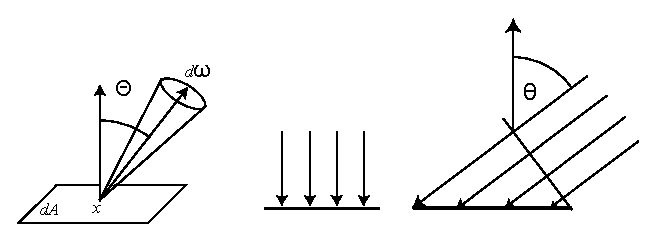
\includegraphics[width=0.85\linewidth]{media/radiance.eps}
	\caption{Definicion de radiancia $L(x,\Theta)$. Flujo radiante emitido por unidad de ángulo solido $dw$ y por unidad de área proyectada $A^\bot$.}
	\label{fig:radiance_fi}
\end{figure}

La radiancia es el término más importante para los propósitos de este trabajo y probablemente lo es también para una cantidad importante de algoritmos y aproximaciones para el cálculo de iluminación global, es esta unidad la que captura la apariencia de los objetos en escena.

\section{Iluminación directa e indirecta}
\label{sec:direct_indirect}
La iluminación directa es aquella que se proyecta sobre la superficie de algún objeto directamente desde las fuentes de luz en la escena. Iluminación indirecta es la luz que proviene de los subsecuentes rebotes de luz originados desde las superficies iluminadas, ya sea esta superficie reflectiva o no \cite{advanced_gi2006}. La composición de ambas resulta en iluminación global.
\section{Representación de Superficies}
\label{sec:surface_rep}

Los materiales interactúan con la luz de distintas maneras. Esto hace que la apariencia de ciertos materiales difiera según la condiciones de la luz en una escena. Algunos materiales parecen espejos mientras que otros son totalmente difusos. Son visualmente distinguible materiales como vidrio, madera o metales. Las propiedades de reflectancia de una superficie afectan la apariencia del objeto \cite{advanced_gi2006}, estos objetos se distinguen por la cantidad de luz reflectada en ciertas direcciones. 

En el caso más general, un rayo de luz entra en algún punto $p$ sobre una superficie en una escena, este rayo de luz tiene una dirección incidente $\Psi$ y puede salir de esta superficie sobre otro punto $q$ con dirección saliente $\Theta$. La función que define esta relación entre la radiancia incidente y la radiancia reflectada se llama \ac{BSSRDF}.

\subsection{Función de Distribución de Reflectancia Bidireccional}
Al asumir que la luz incidente en algún punto $x$ sale del mismo punto $x$ (ignorando la transluminiscencia) las propiedades de reflectancia de una superficie son entonces descritas por una \ac{BRDF}. En la Figura \ref{fig:bssrdf} se puede observar la diferencia entre \ac{BRDF} y \ac{BSSRDF}.

\begin{figure}[H]
	\centering
	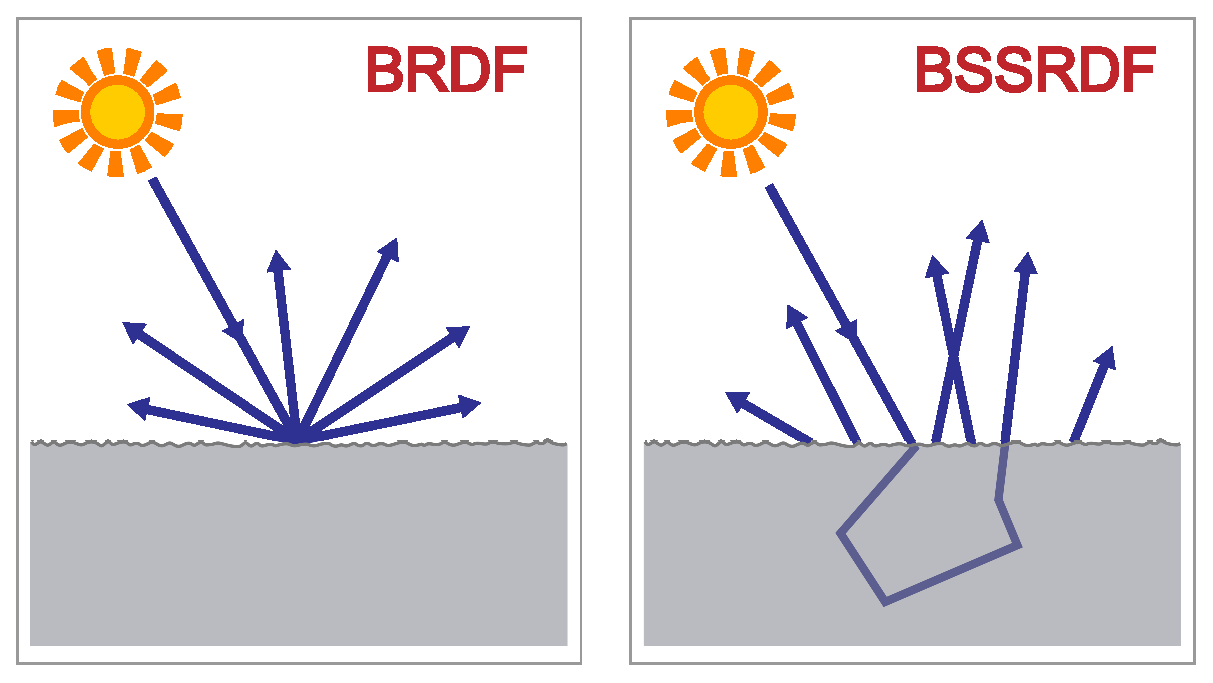
\includegraphics[width=.6\linewidth]{media/brdf_vs.eps}
	\caption
	{
    	Izquierda: BRDF, punto de salida es igual al punto de entrada. Derecha: BSSRDF, se observa como el punto de salida es distinto al de entrada.
	}
	\label{fig:bssrdf}
\end{figure}

La \ac{BRDF} en un punto $x$ se define entonces como la distribución de la radiancia reflectada diferencial en una dirección saliente $\Theta$ y la irradiancia incidente diferencial a través de un ángulo solido $dw_{\Psi}$. La función \ac{BRDF} puede ser escrita de la siguiente forma \cite{advanced_gi2006}:

\begin{equation}
	\begin{split}
        f_{r}(x, \Psi\to\Theta) &= \frac{dL(x\to\Theta)}{dE(x\gets\Psi)}\\
        &= \frac{dL(x\to\Theta)}{L(x\gets\Psi)\cos(N_{x}, \Psi)dw_{\Psi}}
	\end{split}
	\label{eq:brdf_def}
\end{equation} donde $\cos(N_{x}, \Psi)$ es el coseno del ángulo formado entre la normal en el punto $x$ y el vector dirección $\Psi$, también llamado atenuación normal.

\subsubsection{Propiedades de la Función BRDF}

La función BRDF tiene una variada cantidad de importantes propiedades:

\begin{enumerate}
	\item Dimensión: La función BRDF es una función cuatridimensional definida sobre cada punto de una superficie, dos dimensiones corresponden a la dirección entrante y dos a la dirección saliente.
	\item Reciprocidad: El resultado de la función BRDF es el mismo si se intercambian la dirección entrante y la dirección saliente:
    	\begin{equation}
            f_{r}(x, \Psi\to\Theta) = f_{r}(x, \Theta\to\Psi)
    	\end{equation}
	\item Conservación de la energía: La ley de conservación de la energía dicta que la cantidad total de energía reflectada en todas las direcciones debe ser menor o igual a la cantidad de total de energía incidente sobre las superficies: 
    	\begin{equation}
    		\int_{\Omega^{+}}f_{r}(x, \Psi\to\Theta)\cos(N_{x}, \Theta)dw_{\Theta} \leq 1
    	\end{equation}
\end{enumerate}

\subsubsection{Ejemplos de BRDF}
Dependiendo del comportamiento de la \ac{BRDF}, el material se verá como una superficie difusa, como un espejo o como una mezcla de ambos (lustroso o \emph{glossy}). En la Figura \ref{fig:brdf_types} se ilustra estas propiedades. Los tipos de BRDF relevantes para este trabajo serán listados aquí.

\begin{figure}[H]
	\centering
	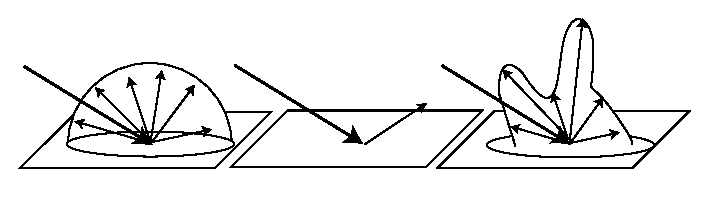
\includegraphics[width=0.85\linewidth]{media/brdfs_types.eps}
	\caption{Ejemplos de superficies: totalmente difusa izquierda, totalmente especular centro, lustrosa (\emph{glossy}) derecha \cite{advanced_gi2006}.}
	\label{fig:brdf_types}
\end{figure}

\paragraph{Superficies Difusas:}
Algunos materiales reflectan la luz de forma uniforme sobre la totalidad de la semiesfera de reflectancia. Esto quiere decir que según la distribución de la irradiancia, la radiancia reflectada es independiente de la dirección de salida. Estos materiales son llamados reflectores difusos y el valor de su \ac{BRDF} es una constante para todos los valores $\Theta$ y $\Psi$. Para un observador un punto sobre una superficie difusa se ve igual desde todas las direcciones \cite{advanced_gi2006}. Para una superficie difusa ideal, la reflexión difusa puede ser representada como:

\begin{equation}
    f_{r}(x, \Psi\leftrightarrow\Theta) = \frac{\rho_{d}}{\pi}
    \label{eq:diffuse_reflection}
\end{equation}

La reflectancia $\rho_{d}$ representa la fracción de la energía incidente que es reflectada en la superficie. Para materiales físicamente correctos, $\rho_{d}$ varía entre 0 y 1.

\paragraph{Superficies Especulares:}
\label{para:speculars}
Superficies especulares perfectas solo reflejan o refractan luz en una dirección específica.
\paragraph{Reflexión Especular:}
La dirección de reflexión puede ser obtenida utilizando la ley de reflexión, esta indica que la dirección de la luz incidente y saliente tienen un ángulo equivalente con la normal de la superficie. Dado que la luz es incidente con respecto a la superficie con vector dirección $\Psi$, y la normal de la superficie es $N$, la luz incidente es reflectada en la dirección $R$:

\begin{equation}
    R = 2(N\cdot\Psi)N - \Psi
    \label{eq:reflectance_direction}
\end{equation}

Un reflector especular perfecto tiene solo una dirección de salida donde la \ac{BRDF} es diferente de $0$, esto implica que el valor de la \ac{BRDF} en esa dirección es infinito.

\paragraph{Superficies Lustrosas:}
La mayoría de las superficies no son ni idealmente difusas ni idealmente especulares, sino que demuestran una combinación de ambas características de reflectancia. Estas superficies son llamadas superficies lustrosas o superficies \emph{glossy}. La \ac{BRDF} que describe esta clase de materiales es usualmente difícil de modelar de forma analítica \cite{advanced_gi2006}.

\subsubsection{Modelos de sombreado.}
Materiales reales puede tener \ac{BRDF}s particularmente complejas. En computación gráfica existen varios modelos que intentan capturar la complejidad de las \ac{BRDF}s. En la siguiente sección se expande sobre ciertos modelos relevantes a este trabajo. Nótese que $\Psi$ es la dirección de la luz (dirección incidente), $\Theta$ es la dirección del observador (dirección saliente) y $N$ la normal de la superficie.

\paragraph{Modelo de Lambert:}
Uno de los modelos más simples, este modelo es ideal para superficies difusas, en este modelo la \ac{BRDF} es una constante como ya fue descrito anteriormente en la ecuación \ref{eq:diffuse_reflection}.

\begin{equation}
    f_{r}(x, \Psi\leftrightarrow\Theta) = k_{d} = \frac{\rho_{d}}{\pi}
    \label{eq:lambert}
\end{equation} donde $\rho_{d}$ es la reflexión difusa.

\paragraph{Modelo de Phong:}
La \ac{BRDF} del modelo de Phong es:

\begin{equation}
    f_{r}(x, \Psi\leftrightarrow\Theta) = k_{s}\frac{(R\cdot \Theta)^n}{N\cdot\Psi} + k_{d}
    \label{eq:phong}
\end{equation} donde el vector reflectado $R$ es calculado con la ecuación \ref{eq:reflectance_direction}.

\paragraph{Modelo de Blinn-Phong:}
\label{para:blinn_phong}
El modelo Blinn-Phong utiliza el vector medio $H$ entre $\Psi$ y $\Theta$ de la siguiente manera:

\begin{equation}
    f_{r}(x, \Psi\leftrightarrow\Theta) = k_{s}\frac{(N\cdot H)^n}{N\cdot\Psi} + k_{d}
    \label{eq:blinn_phong_pr}
\end{equation}

El valor $n$ varía según las propiedades del material. Un mayor valor provee un lóbulo especular más pequeño, simulando superficies lisas y pulidas. En la Figura \ref{fig:blinn_spec_comparison} se puede observar este efecto. En la Figura \ref{fig:brdfs_comparison} se puede observar el resultado de este modelo.

\begin{figure}[H]
	\centering
	\begin{subfigure}[t]{0.25\textwidth}
		\centering
		\captionsetup{justification=centering}
		\includegraphics[width=\linewidth]{media/blinn_10.png}
		\caption*{$n = 10$}
	\end{subfigure}%
	\begin{subfigure}[t]{0.25\textwidth}
		\centering
		\captionsetup{justification=centering}
		\includegraphics[width=\linewidth]{media/blinn_50.png}
		\caption*{$n = 50$}
	\end{subfigure}%
	\begin{subfigure}[t]{0.25\textwidth}
		\centering
		\captionsetup{justification=centering}
		\includegraphics[width=\linewidth]{media/blinn_150.png}
		\caption*{$n = 150$}
	\end{subfigure}%
	\begin{subfigure}[t]{0.25\textwidth}
		\centering
		\captionsetup{justification=centering}
		\includegraphics[width=\linewidth]{media/blinn_350.png}
		\caption*{$n = 350$}
	\end{subfigure}%
	\caption{Distribución especular para distintos valores de $n$ en el modelo Blinn-Phong.}
	\label{fig:blinn_spec_comparison}
\end{figure}

\paragraph{Modelo de Blinn-Phong Modificado:}
\label{para:blinn_phong_mod}
El modelo de Phong a pesar de ser simple este tiene ciertas limitaciones, no es ni conservador de energía ni reciproco y tiene problemas para simular materiales reales. El modelo modificado toma en cuenta algunos de estos problemas:

\begin{equation}
    f_{r}(x, \Psi\leftrightarrow\Theta) = k_{s}(N\cdot H)^n + k_{d}
    \label{eq:blinn_phong}
\end{equation}

\begin{figure}[H]
	\centering
	\begin{subfigure}[t]{0.33\textwidth}
		\centering
		\captionsetup{justification=centering}
		\includegraphics[width=\linewidth]{media/diffuse_bunny.png}
		\caption*{Lambert \ac{BRDF}}
	\end{subfigure}%
	\begin{subfigure}[t]{0.33\textwidth}
		\centering
		\captionsetup{justification=centering}
		\includegraphics[width=\linewidth]{media/specular_bunny.png}
		\caption*{Blinn-Phong \ac{BRDF}\\ especular}
	\end{subfigure}%
	\begin{subfigure}[t]{0.33\textwidth}
		\centering
		\captionsetup{justification=centering}
		\includegraphics[width=\linewidth]{media/diffuse_specular_bunny.png}
		\caption*{Lambert \ac{BRDF} y \\Blinn-Phong \ac{BRDF} especular.}
	\end{subfigure}
	\caption{Composición de Blinn-Phong y Lambert. Se observa como estas afectan la apariencia final de la superficie.}
	\label{fig:brdfs_comparison}
\end{figure}

\subsection{Función de Distribución Normal}
La \ac{NDF} introducida por Alain Fournier \cite{fournier1992d} describe la densidad de las normales como una función de dirección. Funciones gaussianas como la siguiente es una de las posibles formas de una \ac{NDF}.
\begin{equation}
    f(x) = \frac{1}{\sigma\sqrt{2\pi}}e^{-\frac{(x-\mu)^2}{2\sigma^2}}
    \label{eq:ndf_ex1}
\end{equation}

En la función gaussiana el termino $\sigma^2$ es llamado variancia y el termino $\mu$ es llamado media. Tanto el producto como la convolución de dos distribuciones gaussianas es también una distribución gaussiana \cite{tina-2003}.

La función gaussiana puede ser utilizada como una representación direccional. En este caso la media es un vector promedio $D$ del lóbulo gaussiano. Como es descrito en el trabajo de Toksvig para el mipmapping de mapas de normales \cite{Toksvig05}, el valor de $\sigma$ puede ser calculado por la longitud del vector promedio $D$ utilizando la siguiente ecuación:
\begin{equation}
    \sigma^2 = \frac{1-|D|}{|D|}
    \label{eq:gaussia_eq}
\end{equation}

Esto permite obtener lóbulos gaussianos a partir de dos o más vectores para representar su dirección en común. En la Figura \ref{fig:brdf_lobules} se puede observar el lóbulo para una distribución de dos direcciones.

\begin{figure}[H]
	\centering
	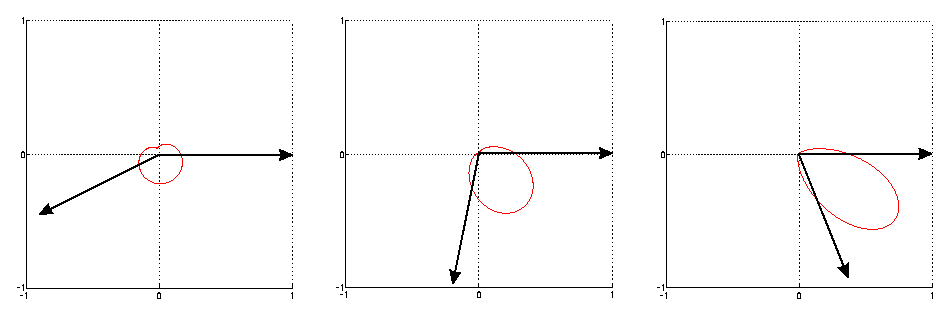
\includegraphics[width=0.85\linewidth]{media/lobes.eps}
	\caption{Ejemplo de lóbulos gaussianos según dos vectores, se puede observar como la forma del lóbulo cambia según la dirección promedio.}
	\label{fig:lobes_example}
\end{figure}

Algunas \ac{BRDF} también pueden describirse como distribuciones gaussianas, las propiedades de producto y convolución se mantienen. Esto se puede observar en la Figura \ref{fig:brdf_lobules}.

\begin{figure}[H]
	\centering
	\begin{subfigure}[t]{0.3\textwidth}
		\centering
		\captionsetup{justification=centering}
		\includegraphics[width=\linewidth]{media/phong_lobule.png}
		\caption*{\ac{BRDF} Phong}
	\end{subfigure}\hfill
	\begin{subfigure}[t]{0.35\textwidth}
		\centering
		\captionsetup{justification=centering}
		\includegraphics[width=\linewidth]{media/BlinnPhonglobules.png}
		\caption*{Gráfica de ambas en coordenadas polares.}
	\end{subfigure}\hfill
	\begin{subfigure}[t]{0.3\textwidth}
		\centering
		\captionsetup{justification=centering}
		\includegraphics[width=\linewidth]{media/blinnphong_lobule.png}
		\caption*{\ac{BRDF} Blinn-Phong}
	\end{subfigure}\hfill
	\caption{Lóbulos especulares para BRDF Phong y Blinn-Phong para un $\Theta$ y $\Psi$ de $\angle 45$, se puede observar cómo estas describen la distribución de la dirección de reflectancia. Como se explica en \ref{para:blinn_phong} el valor de $n$ afecta la forma del lóbulo mientras mayor es este número más fino y largo es el lóbulo especular. Imágenes renderizadas en Disney's BRDF Explorer \cite{brdf_explorer}.}
	\label{fig:brdf_lobules}
\end{figure}

\section{Ecuación de Renderizado}
La ecuación de renderizado fue introducida por Kajiya  en 1986 \cite{kajiya86}. Esta ecuacion describe en cada punto $x$ de una superficie y en cada dirección $\Theta$, la radiancia saliente $L(x\to\Theta)$ en ese punto y esa dirección.

El objetivo de un algoritmo para el cálculo de iluminación global es aproximar el resultado de esta ecuación. En esta ecuación asumimos que no existen medios participantes como objetos translúcidos como ya fue explicado en la sección \ref{sec:surface_rep}. También asumimos que la luz se propaga de forma inmediata por tanto la distribución de la luz, ya en un estado estacionario, se obtiene inmediatamente. 

\subsection{Formulación Hemisférica}
La formulación hemisférica de la ecuación de renderizado es una de las más utilizadas \cite{advanced_gi2006}. Esta formulación se obtiene utilizando la propiedad de conservación de energía en el punto $x$. Asumiendo que $L_{e}(x\to\Theta)$ representa la radiancia emitida por la superficie en el punto $x$ con dirección saliente $\Theta$ y $L_{r}(x\to\Theta)$ representa la radiancia reflectada por la superficie en el punto $x$ en dirección $\Theta$.

Por conservación de energía, el total de la radiancia saliente en un punto y dirección particular es la suma de la radiancia emitida y la radiancia reflectada en este punto de la superficie y dirección. La radiancia saliente $L(x\to\Theta)$ es expresada en términos de $L_{e}(x\to\Theta)$ y $L_{r}(x\to\Theta)$ de la siguiente forma:
\begin{equation}
    L(x\to\Theta) = L_{e}(x\to\Theta) + L_{r}(x\to\Theta)
    \label{eq:reflectance}
\end{equation}
Por la definición de \ac{BRDF} en la ecuación \ref{eq:brdf_def} tenemos que:
\begin{equation}
	\begin{split}
        f_{r}(x, \Psi\to\Theta) &= \frac{dL(x\to\Theta)}{dE(x\gets\Psi)}\\
        L_{r}(x\to\Theta) &= \int_{\Omega_{x}}{f_{r}(x, \Psi\to\Theta)L(x\gets\Psi)\cos(N_{x}, \Psi)dw_{\Psi}}
	\end{split}
	\label{eq:rendering_eq_LR}
\end{equation}
Colocando estas ecuaciones juntas obtenemos la ecuación de renderizado:
\begin{equation}
    L(x\to\Theta) = L_{e}(x\to\Theta) + \int_{\Omega_{x}}{f_{r}(x, \Psi\to\Theta)L(x\gets\Psi)\cos(N_{x}, \Psi)dw_{\Psi}}
    \label{eq:rendering_eq}
\end{equation}

\subsection{Procedimientos}
\label{sub:render_eq_procedures}
En esta sección se explica dos populares procedimientos clásicos para obtener una aproximación a la ecuación de renderizado, esto es una aproximación de la propagación de la luz en una escena. Estas soluciones no están pensadas para tiempos interactivos y su enfoque principal es precisión.

Métodos como elementos finitos y Monte Carlo son los grupos de algoritmos más utilizados para aproximar la ecuación de renderizado. El método de elementos finitos utiliza alguna forma de discretización para reducir la ecuación de renderizado a una ecuación de matrices. Los métodos Monte Carlo muestrean los caminos que siguen los rayos de luz en una escena, generando un estimado estadístico de la apariencia real de la escena. \emph{Radiosity} es una popular aproximación que utiliza el método de elementos finitos. Trazado de rayos y caminos (\emph{ray tracing y path tracing}) son aproximaciones comunes que utilizan el método Monte Carlo \cite{gi_renderingeq}. 

\begin{figure}[H]
	\centering
	\begin{subfigure}{0.24\textwidth}
		\centering
		\captionsetup{width=0.95\textwidth, justification=centering}
		\caption*{Vista desde patch $\alpha$,\\ antes de pasada 1.}
		\includegraphics[width=.95\linewidth]{media/radiosity1_eye.png}
	\end{subfigure}
	\begin{subfigure}{0.24\textwidth}
		\centering
		\captionsetup{width=0.95\textwidth, justification=centering}
		\caption*{Patch $\beta$ debajo de $\alpha$,\\ se observa el sol.}
		\includegraphics[width=.95\linewidth]{media/radiosity1_eye1.png}
	\end{subfigure}%
	\begin{subfigure}{0.24\textwidth}
		\centering
		\captionsetup{width=0.95\textwidth, justification=centering}
		\caption*{Patches iluminados,\\ durante pasada 1.}
		\includegraphics[width=.95\linewidth]{media/radiosity_patch2.png}
	\end{subfigure}%
	\begin{subfigure}{0.24\textwidth}
		\centering
		\captionsetup{width=0.95\textwidth, justification=centering}
		\caption*{Vista desde patch $\alpha$,\\ después de pasada 1.}
		\includegraphics[width=.95\linewidth]{media/radiosity2_eye.png}
	\end{subfigure}
	\label{fig:radiosity1}
\end{figure}%
\begin{figure}[H]
	\centering
	\begin{subfigure}{0.24\textwidth}
		\centering
		\includegraphics[width=.95\linewidth]{media/radiosity1.png}
		\captionsetup{width=0.95\textwidth, justification=centering}
		\caption*{Pasada 1.}
	\end{subfigure}%
	\begin{subfigure}{0.24\textwidth}
		\centering
		\includegraphics[width=.95\linewidth]{media/radiosity2.png}
		\captionsetup{width=0.95\textwidth, justification=centering}
		\caption*{Pasada 2.}
	\end{subfigure}%
	\begin{subfigure}{0.24\textwidth}
		\centering
		\includegraphics[width=.95\linewidth]{media/radiosity3.png}
		\captionsetup{width=0.95\textwidth, justification=centering}
		\caption*{Pasada 3.}
	\end{subfigure}
	\begin{subfigure}{0.24\textwidth}
		\centering
		\includegraphics[width=.95\linewidth]{media/radiosity16.png}
		\captionsetup{width=0.95\textwidth, justification=centering}
		\caption*{Pasada 16.}
	\end{subfigure}
	\caption{Ejemplo de varias pasadas de radiosidad sobre una escena. Fuente: Hugo Elias, \emph{The Workings of a Radiosity Renderer} \cite{hugo2000}.}
	\label{fig:radiosity2}
\end{figure}


\subsubsection{Radiosidad}
\label{subsec:radiosity}

Radiosidad es una aproximación con elementos finitos para el cómputo del transporte de luz global. Esta técnica fue introducida por Goral y otros en 1984 \cite{goral84}. La idea general es discretizar las superficies de la escena en elementos finitos de éstas, estos elementos son usualmente llamados \emph{patches} (parches o trozos) los cuales son utilizados para calcular el transporte de luz entre ellos como se observa en la figura \ref{fig:radiosity2}. Esto conlleva a ciertas implicaciones; de cada \emph{patch} se necesita guardar el valor de radiosidad para las superficies difusas, o la distribución direccional de la luz saliente y entrante para superficies no difusas.

\subsubsection{Trazado de Rayos e Integración Monte Carlo}
\label{subsec:monte_carlo_raytracing}
La ecuación de renderizado puede ser aproximada utilizando el algoritmo de trazado de rayos o \emph{ray tracing}, esta es una técnica basada en integración Monte Carlo. Para aproximar la propagación de la luz sobre un punto se crea un número considerable de muestras en variadas direcciones, luego por cada muestra se evalúa la ecuación de renderizado y el promedio de todos los resultados converge hacia la solución analítica de la ecuación de renderizado sobre ese punto. Para evaluar una muestra la luz incidente desde una dirección tiene que ser calculada, para esto un rayo de luz es enviado en una dirección y la luz emitida desde el primer punto de colisión es calculada evaluando la ecuación de renderizado en este punto.

Ray tracing está dividido en dos categorías: forward y backward. Forward ray tracing consiste en lanzar las trazas/rayos de luz desde las fuentes de luz y usar aquellos que llegan a la cámara. Backward ray tracing por el contrario lanza las trazas/rayos de luz desde la cámara y traza el camino de estos a través de la escena \cite{Arvo86backwardray}.

\begin{figure}[H]
	\centering
	\begin{subfigure}{0.33\textwidth}
		\centering
		\includegraphics[width=.98\linewidth]{media/ray_100s.jpg}
		\captionsetup{width=0.98\textwidth, justification=centering}
		\caption*{100 muestras rayos/píxel,\\ 50 para luces de área.}
	\end{subfigure}%
	\begin{subfigure}{0.33\textwidth}
		\centering
		\includegraphics[width=.98\linewidth]{media/ray_500s.jpg}
		\captionsetup{width=0.98\textwidth, justification=centering}
		\caption*{500 muestras rayos/píxel,\\ 50 para luces de área.}
	\end{subfigure}%
	\begin{subfigure}{0.33\textwidth}
		\centering
		\includegraphics[width=.98\linewidth]{media/ray_1000s.jpg}
		\captionsetup{width=0.98\textwidth, justification=centering}
		\caption*{1000 muestras rayos/píxel,\\ 100 para luces de área.}
	\end{subfigure}
	\caption{Ray tracing sobre una escena, se puede observar mayor calidad y reducción de ruido al aumentar la cantidad de muestras. Fuente: Loc Do, \emph{HW6: Ray Tracing Extension} \cite{locdoraytracing}.}
	\label{fig:ray_tracing_nsamples}
\end{figure}
\section{Técnicas Comunes en Renderizado de Imágenes}

En esta sección se explican técnicas comunes utilizadas en síntesis o renderizado de imágenes que son relevantes para este trabajo.
\subsection{Mapeado de Sombras}
\label{subsec:shadowmapping}
Con la luz es representada en forma de rayo las superficies sombreadas reciben menos rayos de luz ya que estas están ocluidas por otras superficies que se encuentra entre ellas y los emisores de luz. En un pipeline de renderizado general, donde las superficies en escenas son representadas en geometría poligonal, trazar rayos por cada fragmento para comprobar la visibilidad del mismo no es una operación trivial.
\begin{figure}[H]
	\centering
	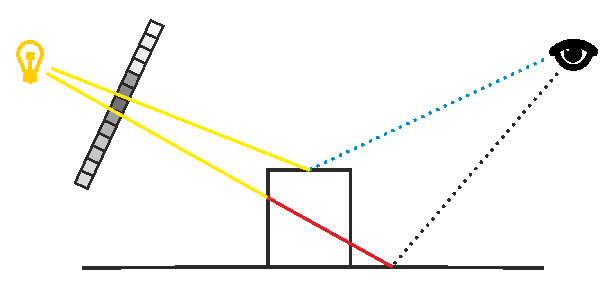
\includegraphics[width=0.85\linewidth]{media/shadow_mapping.eps}
	\caption{La profundidad almacenada en el mapa de sombra (amarillo) es comparada con la profundidad del punto en la superficie desde la luz (rojo).}
	\label{fig:shadow_mapping}
\end{figure}
Los mapas de sombras, presentados inicialmente por Lance Williams en 1978 \cite{Williams:78} presentan una solución simple para el cálculo de visibilidad de un fragmento.

La técnica consiste en proyectar la escena en una textura bidimensional desde la posición y con la dirección de una fuente de luz. La proyección es calculada utilizando una matriz de proyección $P_{l}$. Por cada píxel de esta textura la profundidad de cada fragmento sobre una superficie es almacenada. Esta textura es llamada mapa de sombra.
Una que se pasa a renderizar la escena desde el punto de vista del observador, por cada fragmento con posición $p_{ws}$ en espacio de mundo, la posición en el mapa de sombra $p_{sh}$ es calculada utilizando la siguiente ecuación:
\begin{equation}
    p_{sh} = P_{l} * p_{ws}
    \label{eq:p_to_shadowmap}
\end{equation}
Como se muestra en la figure \ref{fig:shadow_mapping} si la profundidad del fragmento desde la fuente de luz es mayor que el valor almacenado en el mapa de sombra entonces este punto esta sombreado. 

El mapeado de sombras es una solución sencilla y efectiva al problema de pruebas de visibilidad pero este tiene dos mayores problemas. El mapa de sombras está limitado a la resolución de la textura y además este representa una discretización de la profundidad de la escena desde la fuente de luz y esto introduce una variedad de anomalías visuales. A partir de este concepto existe una variedad de algoritmos para el cálculo de sombras que intentan solventar estos problemas.

\subsection{Sombreado Diferido}
\label{sub:deferred_rendering_theory}
En sombreado directo la representación poligonal de la escena es rasterizada y operaciones por píxel como iluminación y sombreado son realizadas por cada fragmento generado por el proceso de rasterización. Esto es poco efectivo cuando consideramos que gran parte de los fragmentos no forman parte de la imagen final.
Con sombreado diferido se pueden realizar estas operaciones por píxel solo sobre los fragmentos visibles. Este concepto está basado en el trabajo de Deering en y otros en 1998 \cite{Deering:1988}. La escena es renderizada solo una vez y varios atributos de la escena son almacenados en buffers. Este buffer es llamado \ac{GBuffer} y fue introducido por Saito y otros en 1990 \cite{Saito:1990}. El contenido general de un G-Buffer es profundidad, albedo y normal, esto puede cambiar según las necesidades de la aplicación. El propósito de almacenar esta información es separar las operaciones que solo son necesarias sobre los fragmentos visibles de la rasterización de toda la escena, de manera que cálculos como iluminación ahora son realizados en otro paso solo sobre cada píxel almacenado en el \ac{GBuffer}.

\begin{figure}[H]
	\centering
	\begin{subfigure}[t]{0.32\textwidth}
		\centering
		\captionsetup{justification=centering}
		\includegraphics[width=\linewidth]{media/engine-Context2-Texture13level0.png}
		\caption*{Normales.}
	\end{subfigure}%
	\hspace{0.01\textwidth}
	\begin{subfigure}[t]{0.32\textwidth}
		\centering
		\captionsetup{justification=centering}
		\includegraphics[width=\linewidth]{media/engine-Context2-Texture14level0.png}
		\caption*{Albedo.}
	\end{subfigure}%
	\hspace{0.01\textwidth}
	\begin{subfigure}[t]{0.32\textwidth}
		\centering
		\captionsetup{justification=centering}
		\includegraphics[width=\linewidth]{media/engine-Context2-Texture17level0.png}
		\caption*{Profundidad.}
	\end{subfigure}%
	\caption{El contenido de un buffer de geometría.}
	\label{fig:gbuffer}
\end{figure}

\subsection{Voxelización}
\label{sec:voxelization}
Un \emph{voxel} o a veces llamado píxel volumétrico representa una muestra singular o punto de data sobre un grid regular en un espacio 3-dimensional. Esta data puede ser cualquier valor definido por la aplicación o incluso múltiples valores. 

El proceso de generar superficies discretas en una representación volumétrica a través de vóxeles se le llama voxelización.

\begin{figure}[H]
	\centering
	\begin{subfigure}{0.33\textwidth}
		\centering
		\includegraphics[width=.6\linewidth]{media/rigid01.pdf}
		\captionsetup{width=0.95\textwidth}
		\caption{Grid regular del vóxeles.}
	\end{subfigure}%\\
	\begin{subfigure}{0.33\textwidth}
		\centering
		\includegraphics[width=.6\linewidth]{media/rigid02.pdf}
		\captionsetup{width=0.95\textwidth}
		\caption{Superficie en el grid.}
	\end{subfigure}%\\
	\begin{subfigure}{0.33\textwidth}
		\centering
		\includegraphics[width=.6\linewidth]{media/rigid03.pdf}
		\captionsetup{width=.95\textwidth}
		\caption{Superficie en vóxeles.}
	\end{subfigure}%
	\caption{Representación de una superficie en vóxeles con voxelización fina.}
	\label{fig:rigid_grid}
\end{figure}

Se puede distinguir el proceso de voxelización de superficies en dos clases: voxelización fina con separabilidad factor 6 y voxelización conversadora con todos los vóxeles que tocan la superficie activos o separabilidad factor 26. En el trabajo de Huang y otros en 1998 \cite{Huang:1998:AMV:288126.288181} se describe el proceso de voxelización y terminología con mayor detalle. También existen cuatro tipos de enfoques en voxelización:

\begin{itemize}
	\label{list:voxelization_types}
	\item \textbf{Voxelización binaria:} Cada vóxel sólo almacena si hay geometría presente o no.
	\item \textbf{Voxelización multi-valor:} Cada vóxel puede almacenar múltiples valores de data arbitraria como opacidad, normal, etc.
	\item \textbf{Voxelización de contorno:} Sólo se voxeliza la superficie o contorno de los objetos.
	\item \textbf{Voxelización sólida:} Además de la superficie también se voxeliza el interior del objeto.
\end{itemize}

\section{Iluminación Global en Tiempo Real.}
\label{sec:interactive_gi_takes}
En esta sección se examinan algunos algoritmos para el cálculo de iluminación global en tiempos interactivos o \emph{real-time}. Iluminación indirecta con trazado de conos y vóxeles es revisada con detalle ya que esta técnica es de particular interés para este trabajo.

\subsection{Luces Puntuales Virtuales}
Una variedad de algoritmos para el cálculo de iluminación global se inspiran o hacen uso del concepto de \ac{VPL}. Este trabajo fue presentado por Keller en 1997 \cite{Keller:1997}.

\begin{figure}[H]
	\centering
	\begin{subfigure}[h]{0.35\textwidth}
		\centering
		\captionsetup{justification=centering}
		\includegraphics[width=\linewidth]{media/vpl1.png}
		\caption*{Generación de luces virtuales puntuales}
	\end{subfigure}
	\hspace{0.1\textwidth}
	\begin{subfigure}[h]{0.35\textwidth}
		\centering
		\captionsetup{justification=centering}
		\includegraphics[width=\linewidth]{media/vpl2.png}
		\caption*{Aproximación de iluminación acumulada sobre un punto.}
	\end{subfigure}
	\caption{Pasos del algoritmo \ac{VPL} para la aproximación de iluminación indirecta. Fuente: Dachsbacher y otros, \emph{Scalable Realistic Rendering with Many-Light Methods} \cite{Dachsbacher2014ManyLights}.}
	\label{fig:vpl_passes}
\end{figure}


En este algoritmo se aproxima la radiancia reflectada en escena utilizando un conjunto de luces virtuales. La radiancia que llega a un punto $x$ es aproximada por la radiancia que proviene de las luces virtuales. Pruebas de visibilidad para cada una de estas luces son realizadas utilizando técnicas de sombreado estándar y la radiancia proveniente de cada una de estas es almacenada en un buffer de acumulación.
Las luces virtuales son generadas a partir de partículas lanzadas por las fuentes de luz principales utilizando la secuencia de Halton para el muestreo. En un principio, un numero $n$ de partículas son generadas, como no toda la radiancia es absorbida algunas de estas partículas son reflejadas. Luego del primer rebote, uno numero $p'n$ de partículas son reflejadas. Luego de $j-1$ reflexiones $p'^j$ son reflejadas. El numero $p'$ es descrito por la siguiente ecuación.
\begin{equation}
    p' = \frac{\sum_{k=1}^{K} p_{d,k}|A_{k}|}{\sum_{k=1}^{K}|A_{k}|}
    \label{eq:reflected_vpls}
\end{equation}
Donde la escena es compuesta por $K$ elementos de superficie $A_{k}$ con una reflectividad promedio de $p_{d,k}$.

\subsection{Mapas de Sombras Reflexivo}
Otra técnica utilizada en varios algoritmos de iluminación global es \ac{RSM} o \emph{reflective shadow maps}. La técnica es \ac{RSM} presentada por Dachsbacher y otros en 2005 \cite{Dachsbacher:2005}.  Esta técnica está inspirada en mapeado de sombras como ya fue explicado anteriormente en \ref{subsec:shadowmapping}, se utiliza proyección desde la fuente de luz para determinar el primer rebote de luz. Al renderizar la escena desde el punto de vista de la fuente de luz, se entiende que todos los fragmentos en el mapa de sombras son los únicos fragmentos involucrados en el primer rebote de luz. En \ac{RSM} cada uno de los píxeles en el mapa de sombras es considerado una fuente de luz. Por cada píxel $p$ además de la profundidad $d_{p}$, se necesita almacenar posición $x_{p}$, normal $n_{p}$, y el flujo de radiancia reflectada $\Theta_{p}$.

\begin{figure}[H]
	\centering
	\begin{subfigure}[t]{.24\linewidth}
		\centering
		\captionsetup{justification=centering}
		\includegraphics[width=\linewidth]{media/rsmd.png}
		\caption*{Profundidad.}
	\end{subfigure}
	\begin{subfigure}[t]{.24\linewidth}
		\centering
		\captionsetup{justification=centering}
		\includegraphics[width=\linewidth]{media/rsmp.png}
		\caption*{Posición.}
	\end{subfigure}
	\begin{subfigure}[t]{.24\linewidth}
		\centering
		\captionsetup{justification=centering}
		\includegraphics[width=\linewidth]{media/rsmn.png}
		\caption*{Normal.}
	\end{subfigure}
	\begin{subfigure}[t]{.24\linewidth}
		\centering
		\captionsetup{justification=centering}
		\includegraphics[width=\linewidth]{media/rsmf.png}
		\caption*{Flujo de radiancia.}
	\end{subfigure}
	\caption{Mapas utilizados por \ac{RSM}. Fuente: Dachsbacher y otros, \emph{Reflective Shadow Maps} \cite{Dachsbacher:2005}.}
	\label{fig:rsm_fbo}
\end{figure}

Si asumimos que todas las superficies son reflectores difusos, la intensidad de la radiancia emitida en una dirección $\omega$ desde un píxel del \ac{RSM} es descrita por la siguiente ecuación.

\begin{equation}
    I_{p}(\omega) = \Theta_{p}max(0, n_{p} \cdot {w})
    \label{eq:rsm_radiance}
\end{equation}

La iluminación indirecta de un punto se calcula sumando todas las intensidades de todos los píxeles (considerados ahora como luces) en el \ac{RSM} visibles. Calcular esto es costoso, por tanto en vez sumar todos los píxeles visibles al punto se toma cierta cantidad de muestras del \ac{RSM}. La posición del punto iluminado $x_{p}$ es proyectado sobre el \ac{RSM} y las muestras son seleccionadas alrededor de esta posición proyectada. La densidad de las muestras decrece con la distancia cuadrada de la posición proyectada al punto iluminado. Esto asume que dos superficies cercanas proyectadas al \ac{RSM} también son cercanas en el \ac{RSM}. También se asume que la muestra es directamente visible desde la superficie iluminada.

\subsection{Volúmenes de Propagación de Luz en Cascada}
\Ac{CLPV} o \emph{Cascaded Light Propagation Volumes} presentando por Kaplanyan y otros en 2010 \cite{Kaplanyan:2010} es un algoritmo para el cálculo de iluminación indirecta en tiempo real.

\begin{figure}[H]
	\centering
	\includegraphics[width=0.85\linewidth]{media/lpvresult.png}
	\caption{Iluminación global para la escena \emph{Sponza} utilizando volúmenes de propagación de luz. Composición final arriba y solo iluminación indirecta abajo. Fuente: Kaplanyan y otros, \emph{Cascaded Light Propagation Volumes for Real-time Indirect Illumination} \cite{Kaplanyan:2010}}
	\label{fig:lvp_results}
\end{figure}

\begin{wrapfigure}[11]{l}{0.3\linewidth}
	\centering
	\includegraphics[width=0.90\linewidth]{media/g4957.png}
	\caption{Cuadriculas de \\ propagación anidadas, las cuadriculas se solapan.}
	\label{fig:nested_lpv}
\end{wrapfigure}
Este método simula el transporte de luz utilizando técnicas similares en algoritmos para simulación de fluidos basados en cuadriculas \cite{Crane07} tridimensionales. La intensidad de luz es almacenada en una cuadricula y de forma iterativa cada celda transfiere la intensidad de la luz a sus vecinos. Esta cuadricula es llamada \ac{LPV}. Esta luz puede ser bloqueada por la geometría de la escena, la cual es obtenida de otra cuadricula llamada \ac{GV}. Para mejorar el rendimiento del algoritmo y reducir el consumo de memoria se utiliza un conjunto de cuadriculas anidadas. Para los objetos cercanos al observador la iluminación indirecta es calculada utilizando una cuadricula mucho más fina.

Primero por cada fuente de luz, es necesario renderizar un \ac{RSM}. Cada texel del \ac{RSM} es considerado una \ac{VPL}. La intensidad del \ac{VPL} es acumulada y almacenada como un harmónico esférico dentro de las celdas de la cuadricula.

Para una correcta propagación de la luz el algoritmo necesita conocer la geometría de la escena. Por esto de la misma manera en la que se almacena la intensidad de la luz también se almacena una representación de la escena en una cuadricula. Esta representación es guardada sobre el \ac{GV}. Esta cuadricula es trasladada por mitad de tamaño de celda unidades con respecto al \ac{LPV}, esto asegura que el centro de todas las celdas del \ac{GV} queden en las esquinas del \ac{LPV}. Para conocer segmentos de geometría se utiliza un \ac{GBuffer} y las fuentes de luz de los \ac{RSM}s.


\begin{figure}[H]
	\centering
	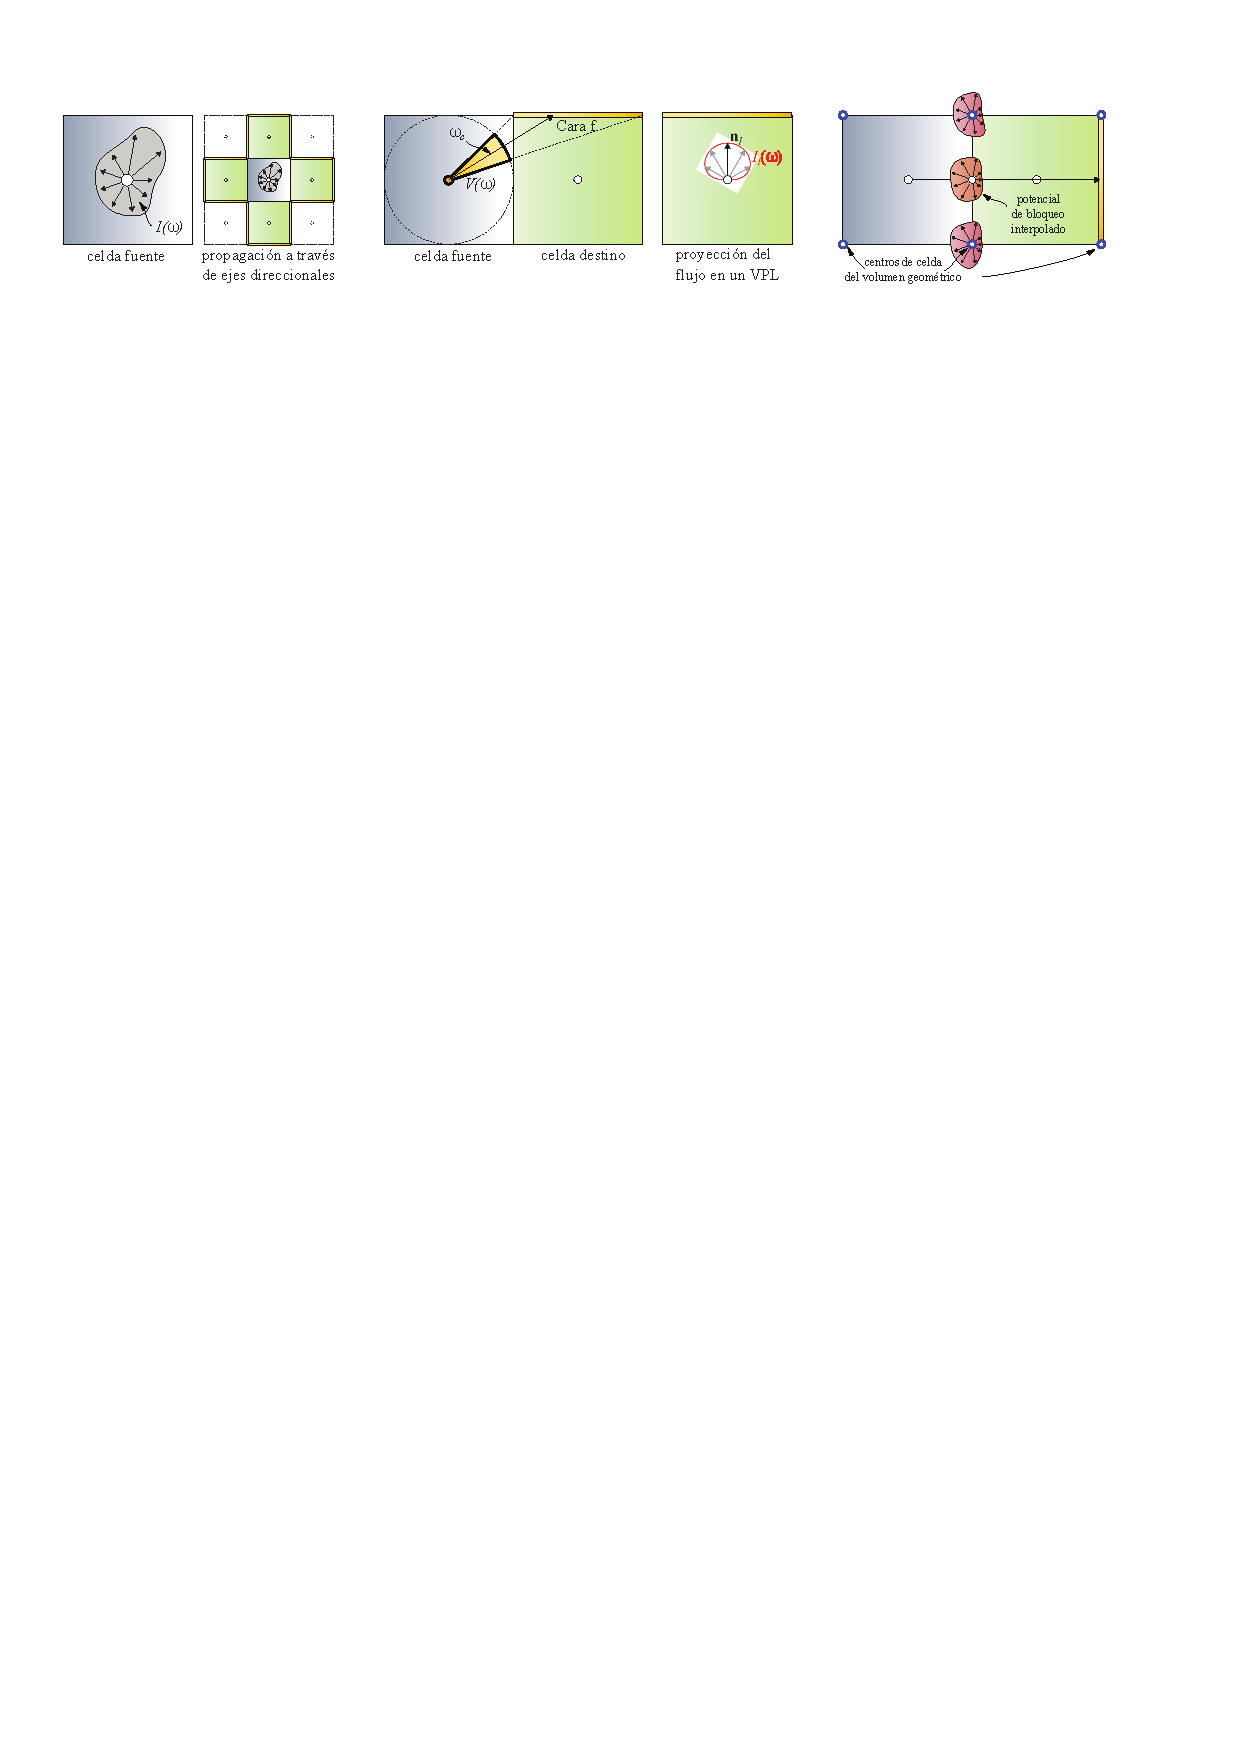
\includegraphics[width=\linewidth]{media/lpv_explain.png}
	\caption{Izquierda: Cada celda del \ac{LPV} almacena la intensidad de luz que es propagada desde la celda fuente. Centro: El flujo es calculado sobre cada cara de la celda destino para preservar información direccional. Derecha: Oclusión borrosa o \emph{fuzzy} almacenando una representación volumétrica de la escena \cite{Kaplanyan:2010}.}
	\label{fig:lpv_explain}
\end{figure}

La propagación de luz se realiza de forma iterativa. La intensidad de luz en cada iteración es propagada a 6 vecinos por celda según eje direccional principal. Primero por cada celda adyacente el flujo de radiancia incidente por cada una de las celdas es calculado. Luego el flujo incidente de cada celda es transformado en emitancia radiante. Esto se logra creando \ac{VPL}s, cada una de estas luces virtuales colocadas sobre una de las caras de la celda y emitiendo un flujo radiancia similar el flujo de radiancia de la celda. Estas \ac{VPL} son acumuladas dentro del \ac{LPV} de nuevo y almacenadas como esféricos harmónicos utilizando el mismo proceso de inyección del primer paso. 

\subsection{Iluminación Indirecta con Trazado de Conos y Vóxeles}
\label{sub:voxel_cone_tracing_orig}
Este algoritmo es presentado por Crassin y otros en 2011 \cite{CNSGE11b} para el cálculo de iluminación indirecta utilizando trazado de conos contra vóxeles o \emph{Indirect Illumination Using Voxel Cone Tracing}. En este técnica se utiliza una estructura de árbol disperso o \emph{sparse} para almacenar ya filtrados los valores necesarios para el cálculo de iluminación indirecta en vóxeles. Este árbol es una representación tridimensional de la escena por tanto cada nodo tiene ocho hijos que representan las ocho particiones de un cubo en partes más pequeñas de forma uniforme. Esta clase de estructuras son llamadas \emph{octrees}. La estructura dispersa requiere menor consumo de memoria ya que solo los vóxeles necesarios son almacenados.

\begin{figure}[H]
	\centering
	\includegraphics[width=0.9\linewidth]{media/givoxels_sponzanew1.png}
	\caption{Escena \emph{Sponza} renderizada utilizando con \acl{VCT} para la iluminación indirecta. Fuente: Cyril Crassin y otros, \emph{Interactive Indirect Illumination Using Voxel Cone Tracing} \cite{CNSGE11b}.}
	\label{fig:givoxels_sponzanew1}
\end{figure}

El algoritmo comprende varios pasos. Primero la información de la luz y escena son almacenados en las hojas de la estructura de árbol, este es el nivel más fino de la jerarquía. Luego estos valores son filtrados dentro del árbol disperso hacia todos los niveles de la jerarquía hasta llegar a la raíz. En un último paso para el cálculo de iluminación indirecta por cada fragmento, los valores dentro de esta jerarquía son recolectados sobre una semiesfera. En algoritmos como ray tracing esta recolección de valores es lenta y es realizada por muchos rayos. Es de notar que todos estos rayos trazados sobre la semiesfera son direccional y espacialmente coherentes. \ac{VCT} hace uso de este concepto para discretizar muchos rayos en simples conos.

\subsubsection{Construcción del Octree de Vóxeles}
El algoritmo está pensando para funcionar con escenas dinámicas. Sin embargo las escenas son divididas entre partes dinámicas y estáticas para acelerar el proceso de voxelización con objetos dinámicos.

Primero la escena es renderizada utilizando proyección ortogonal. Cada triangulo es proyectado sobre uno de los ejes principales, este eje es seleccionado según la normal del triángulo, esto se hace para maximizar el área visible del triángulo según con respecto al eje. Cada fragmento producto de esta proyección es almacenado en una lista de vóxeles-fragmentos junto a parámetros como posición en escena, normal y color. Para saber la cantidad de elementos que esta lista debe almacenar se debe realizar una pasada antes contando el número de fragmentos con un contador atómico.

\begin{wrapfigure}{l}{0.4\linewidth}
	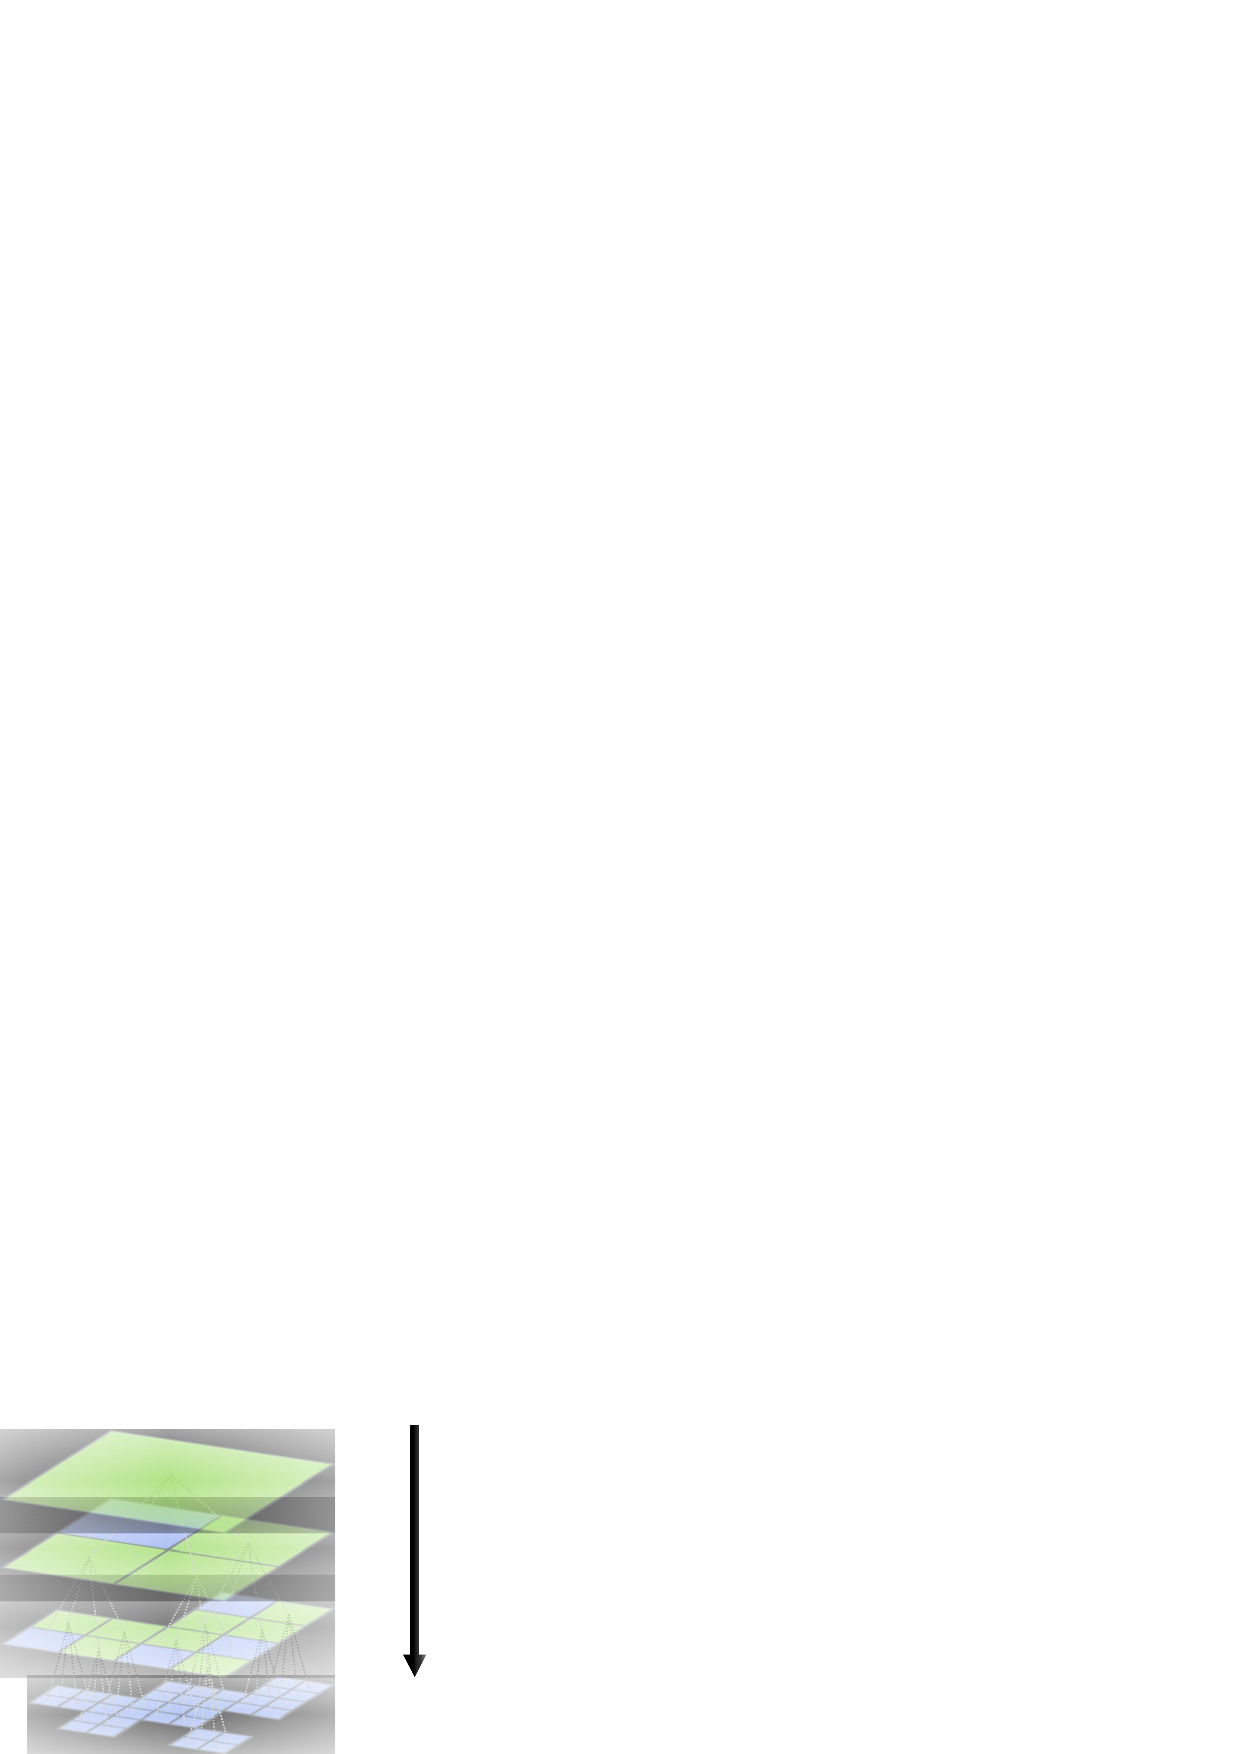
\includegraphics[width=0.95\linewidth]{media/miplevels.png}
	\caption{Descripción gráfica del proceso de subdivisión del octree.}
	\label{fig:miplevels}
\end{wrapfigure}

Una vez llena la lista de vóxeles-fragmentos. Se genera un hilo de procesamiento por cada fragmento en la lista. Los fragmentos son introducidos en el árbol disperso que inicialmente solo tiene un nodo raíz. Cada vez que un nodo de este octree necesita ser dividido un nuevo nodo es creado y se almacena sobre memoria ya reservada en la \ac{GPU}. La posición del nodo en memoria es determinada por un contador atómico, el cual se incrementa con cada nuevo nodo. Al inicio del proceso de subdivisión de los nodos es de esperar una gran cantidad de colisiones entre hilos, por esto cada nodo tiene asociado un símbolo mutex.

\subsubsection{Contenido de un Vóxel}
\label{subsub:voxelcontent_orig}

El algoritmo está diseñado para hacer uso de filtrado tri-linear por hardware. Sin embargo dos vóxeles vecinos no necesariamente están posicionados de forma subsecuente en memoria. Por esto cada nodo contiene un bloque o \emph{brick}. Este bloque representa el entramado $3^3$ de la celda, donde estas celdas se encuentran en las esquinas de los hijos del nodo.

Cada vóxel representa varios parámetros. Entre ellos color, opacidad, normal, intensidad, etc.

\begin{figure}[H]
	\centering
	\includegraphics[width=0.3\linewidth]{media/bricks_vct.png}
	\caption{Bloques y nodos, los valores de los bloques se encuentran en las esquinas para rápido acceso y filtrado \cite{CNSGE11b}.}
	\label{fig:bricks_vct}
\end{figure}

\subsubsection{Filtrado Mip-mapping}
\label{subsub:mipmaping_orig}
Inicialmente cada uno de estos parámetros es almacenado dentro de las hojas del árbol disperso. Luego de forma iterativa estos valores son filtrados desde los niveles más bajos a los niveles más altos de la jerarquía, este proceso es llamado \emph{mip-mapping}. Cada nodo de un bloque es filtrado a partir de las $3^3$ celdas del nivel anterior en jerarquía. Para calcular el valor filtrado sobre el actual nodo el algoritmo promedia los valores de los nodos en el nivel anterior. Al calcular el valor filtrado cada vóxel debe ser pesado con la inversa de su multiplicidad, resultando en un kernel gaussiano de $3^3$. 

\subsubsection{Trazado de Conos y Vóxeles}
Una vez que el árbol disperso esta filtrado y completo este es utilizado para el cálculo de iluminación indirecta. Por cada fragmento un conjunto de conos es generado. La dirección y apertura de cada cono es determina por la \ac{BRDF} del material en ese fragmento. Por ejemplo la \ac{BRDF} Blinn-Phong vista en \ref{para:blinn_phong} puede ser descompuesta como un lóbulo ancho para la parte difusa y un lóbulo especular. Para el lóbulo difuso varios conos son generados orientados por la semiesfera con apertura y dirección maximizada a tal manera que los conos cubran parte de la misma. Para el lóbulo especular se genera un solo cono con una apertura que varía según el termino $n$ de la \ac{BRDF} Blinn-Phong. El cono especular tiene como dirección la dirección de la luz incidente reflectada $R$ visto en \ref{para:speculars}.

\begin{figure}[H]
	\centering
	\begin{subfigure}[t]{.33\linewidth}
		\centering
		\captionsetup{justification=centering}
		\includegraphics[width=\linewidth]{media/lambert.png}
		\caption*{\ac{BRDF} Lambert.}
	\end{subfigure}\hfill
	\begin{subfigure}[t]{.33\linewidth}
		\centering
		\captionsetup{justification=centering}
		\includegraphics[width=\linewidth]{media/blinn_phong_spec.png}
		\caption*{Especular de \ac{BRDF} Blinn-Phong.}
	\end{subfigure}\hfill
	\begin{subfigure}[t]{.33\linewidth}
		\centering
		\captionsetup{justification=centering}
		\includegraphics[width=\linewidth]{media/blinn_phong.png}
		\caption*{\ac{BRDF} especular Blinn-Phong mas Lambert.}
	\end{subfigure}
	\caption{Graficas en coordenadas polares de la BRDF Lambert, especular Blinn-Phong y composición de ambas.}
	\label{fig:brdf_cones}
\end{figure}

El algoritmo utiliza trazado de conos aproximados para recolectar la intensidad de la luz incidente sobre el fragmento. Los valores son recolectados de varias muestras a través del recorrido del cono. Por cada muestra se examina el árbol disperso de vóxeles. El nivel del árbol a examinar es determinado por el diámetro del cono en esa posición.

\subsubsection{Filtrado Anisótropo de Vóxeles.}
\label{subsub:aniso_voxels_orig}
A pesar de que el filtrado gaussiano es suficiente para proveer resultados visuales coherentes, algunos problemas de calidad visual pueden ocurrir bajo ciertas condiciones. El primer problema se conoce como el problema de la pared rojo-verde. Al promediar valores dentro del octree si dos vóxeles opacos con diferentes colores provenientes de por ejemplo, dos paredes planas, el color resultante del vóxel describe ambas paredes como si estas fueran transparentes. Otro problema resulta también de promediar opacidad entre vóxeles totalmente transparentes y vóxeles totalmente opacos, resultando un valor filtrado semitransparente. Esto puede resultar en fugas de luz a través de la geometría en la escena.
Para solventar este problema se realiza una representación anisótropa de los vóxeles durante el proceso de mip-mapping. En vez de tener un solo canal de valores filtrados sin dirección, ahora los valores serán filtrados de forma direccional, almacenando 6 canales por cada eje positivo y negativo. Un valor direccional es calculado realizando un paso de integración volumétrica en profundidad y promediando los cuatro valores direccionales para obtener el valor resultante según una dirección.

\begin{figure}[H]
	\centering
	\includegraphics[width=0.95\linewidth]{media/image23177.png}
	\caption{La caja izquierda describe el proceso de mipmapping de vóxeles sin (izquierda) y con (derecha) filtrado anisótropo. Los pasos para la integración direccional en la caja central. La caja derecha muestra la diferencia entre un vóxel anisótropo como resultado final versus un vóxel isotrópico filtrado por kernel gaussiano \cite{CNSGE11b}.}
	\label{fig:vct_anisofiltering}
\end{figure}

\subsubsection{Captura de Iluminación Directa}
\label{subsub:voxel_capture}
Para el cálculo de iluminación indirecta es necesario describir como la radiancia incidente es almacenada en los nodos del árbol. Este proceso está inspirado en \ac{RSM}, donde la escena es renderizada desde el punto de vista de la fuente de luz y se utiliza rasterización estándar para almacenar las posiciones de los fragmentos en una textura. Cada píxel en esta textura representa un fotón que rebota en escena. Esta textura se le llama mapa de luz-vista o \emph{light-view map}. Luego de generar este mapa es necesario almacenar los fotones en el árbol octree. Los fotones son almacenados como una distribución direccional y energía proporcional al casquete esférico del ángulo solido del píxel visto desde la luz.

El procesamiento de la textura de fotones sobre el árbol se realiza en el procesador de fragmentos o \emph{fragment shader}. Como usualmente la dimensión del \emph{light-view map} es mayor a la resolución de la cuadricula de vóxeles se puede asumir que los fotones serán almacenados directamente en las hojas del árbol octree. Además, los fotones siempre pueden ser almacenados en el nivel más fino de detalle en la representación con vóxeles porque estos describen información de la superficie geométrica. Es posible que muchos fotones terminen sobre un mismo vóxel, por esto es necesario utilizar adicción atómica para garantizar coherencia entre los hilos generados por cada fragmento.

  % propuesta de aplicacion
  \chapter{Solución Propuesta}
\label{chap:proposal}

Un componente de considerable importancia en la composición de imágenes realistas es la iluminación. Para el cálculo de iluminación directa bajo el pipeline de renderizado estándar ya se tienen décadas de estudio y distintas técnicas que permiten tiempos de renderizado muy cortos en hardware moderno. En contraste el cálculo de iluminación indirecta sigue siendo una tarea computacionalmente compleja. 

Para el cálculo de iluminación indirecta existen varios procedimientos muchos de estos inspirados en los ya explicados en la sección \ref{sub:render_eq_procedures}. Sin embargo estos procedimientos no están pensados para renderizado en tiempo real. En la sección \ref{sec:interactive_gi_takes} examinamos algunas aproximaciones para el cálculo de iluminación indirecta en tiempo real, estas técnicas explotan ciertas características de hardware o recursos del pipeline de renderizado.

Nuestra implementación para el cálculo de iluminación global en tiempo real está fuertemente inspirada por el trabajo de Crassin y otros en 2011 \cite{CNSGE11b}. Este trabajo ya fue examinado en la sección \ref{sub:voxel_cone_tracing_orig}. La técnica fue escogida por que además de reflexión difusa también permite el cálculo de superficies lustrosas con reflexión especular a diferencia de otras técnicas como \ac{LPV} que solo permiten reflexión difusa. Una ventaja de esta aproximación es que los valores de radiancia ya se encuentran almacenados sobre una representación con vóxeles. Esto acelera el cálculo de luz incidente bajo el esquema de integración Monte Carlo visto en la sección \ref{subsec:monte_carlo_raytracing}, en este caso los conos permiten realizar una cruda aproximación de un grupo de rayos. Además de esto el algoritmo puede ser usado en escenas totalmente dinámicas.

\section{Voxelización} % (fold)
\label{sec:voxelizacion}
El trazado de conos contra geometria poligonal compleja es costoso. Encontrar los puntos de interseccion entre un cono y un poligono es mas complejo que intersecciones rayo-poligono, ademas de esto un solo cono podria intersectar muchos poligonos.

Para simplificar el trazado de conos se utiliza una discretizacion de la escena en forma de voxeles. Esta representacion puede ser filtrada a niveles mas bajos de detalle. Esto nos permite aproximar el efecto de extender la apertura del cono utilizando cada vez un nivel de detalle mas bajo a traves del recorrido del mismo.

\begin{figure}[H]
	\centering
	\begin{subfigure}[b]{.32\linewidth}
		\centering
		\captionsetup{justification=centering}
		\includegraphics[width=\linewidth]{media/finals/albedo_v256.png}
	\end{subfigure}%
	\hspace{0.01\textwidth}
	\begin{subfigure}[b]{.32\linewidth}
		\centering
		\captionsetup{justification=centering}
		\includegraphics[width=\linewidth]{media/finals/albedo_v128.png}
	\end{subfigure}%
	\hspace{0.01\textwidth}
	\begin{subfigure}[b]{.32\linewidth}
		\centering
		\captionsetup{justification=centering}
		\includegraphics[width=\linewidth]{media/finals/albedo_v64.png}
	\end{subfigure}%
	\caption{Distintos niveles de detalle de una escena voxelizada.}
	\label{fig:voxelization_details}
\end{figure}

Este proceso de voxelizacion para las partes dinamicas de la escena debe ser realizado cada vez que se realiza un cambio sobre alguna superficie que pertenece a algun objeto dinamico en la escena. Por esta razon se requiere un algoritmo de voxelizacion de alto rendimiento para mantener tiempos interactivos.

\subsection{Voxelizacion Conservativa} % (fold)
\label{sub:voxelizacion_conservativa}
Nuestra implementacion realiza voxelizacion conservativa de geometria de alto rendimiento totalmente por \ac{GPU} explotando caracteristicas del pipeline de renderizado de OpenGL. Para esto se implemento el algoritmo de voxelizacion utilizando rasterizacion en hardware explicado en el libro OpenGL Insights por Cyril Crassin y Simon Green en \empty{Octree-Based Sparse
Voxelization Using the GPU
Hardware Rasterizer} \cite{CozziRiccio12}. 

% Esta tecnica utiliza el \emph{geometry shader} y proyeccion ortogonal del triangulo por cada eje para encontrar la maxima area de voxelizacion. La voxelizacion conservativa se logra expandiendo cada vertice del triangulo segun los planos perpendiculares al triangulo por cada par de vertices del mism

Este algoritmo esta basado en el trabajo de Zhang y otros en 2007 \cite{zhang2007conservative} para la voxelization conservativa utilizando la \ac{GPU} y el trabajo de Hasselgren y otros en 2005 \cite{hasselgren2005conservative} sobre rasterizacion conservativa.

Para maximizar el area de rasterizacion la idea es proyectar cada triangulo utilizando proyeccion ortogonal por cada eje direccional. El eje dominante es escogido segun la normal del plano definido por los vertices del triangulo.

\begin{figure}[H]
	\centering
	\captionsetup{justification=centering}
	\includegraphics[width=\linewidth]{media/voxelization_pipeline.eps}
	\captaion{Pipeline de voxelizacion utilizado en nuestra implementacion.}
\end{figure}
 
Por cada triangulo proyectado es necesario generar un poligono delimitante un poco mas grande que el triangulo para garantizar la voxelizacion conservativa. Este poligono debe permitir que por cualquier triangulo proyectado tocando un pixel este va obligatoriamente a tocar el centro de este pixel por tanto el pipeline de rasterizacion generara fragmentos para este traingulo. Este poligono se genera expandiendo cada vertice del triangulo hacia afuera utilizando el \emph{geometry shader}. El poligono delimitante no sobreestima la cobertura del triangulo por tanto este no tiene forma de triangulo. Los fragmentos excedentes de este poligono son descartados en el \emph{fragment shader} utilizando un cuboide delimitante.


% subsection voxelizacion_conservativa (end)
% section voxelizacion (end)

\subsection{Voxelización Dinámica} % (fold)
\label{sub:voxelizacion_dinamica}

% subsection voxelizacion_dinamica (end)

\section{Sombreado de Vóxeles} % (fold)
\label{sec:sombreado_de_voxeles}
Para el cálculo de iluminación indirecta es necesario sombrear cada vóxel. El proceso de sombreado de vóxeles nos permite almacenar la radiancia incidente sobre la escena discretizada en vóxeles. En el trabajo de Crassin esto se hace calculando la iluminación directa sobre los vóxeles utilizando \emph{light-view maps} por cada fuente de luz como ya fue explicado en la sección \ref{subsub:voxel_capture}. Este proceso puede ser ineficiente tanto en consumo de memoria como en rendimiento cuando se considera una escena con muchas luces ya que por cada luz se debe realizar este proceso y se debe tener un mapa de luz-vista asociado (seis para luces puntuales). Otra desventaja de este método es la dependencia del rendimiento con la resolución del mapa de luz-vista. Al aumentar la resolución de esta textura también se aumenta el número de colisiones por cada fragmento que desear escribir sobre un mismo vóxel.

Nuestra implementación utiliza \emph{compute shaders} o el procesador de computo en la \ac{GPU} para el sombreado difuso de cada vóxel. Para calcular el termino difuso sobre un fragmento utilizando la \ac{BRDF} de Lambert (ecuación \ref{eq:lambert}) necesitamos saber el valor de $\rho_{d}$ el cual ya es almacenado en nuestro volumen albedo. Esta constante luego debe ser multiplicada por el $\cos(N_{x}, \Psi)$ para calcular la reflexión difusa de este fragmento. Por esto también se crea un volumen de normales. El vector $\Psi$ se obtiene a partir la dirección de cada fuente de luz en escena.

Para fuentes de luz con dirección no uniforme como luces puntuales o focales es además necesario saber la posición de este fragmento. Siendo cada vóxel una representación discreta de un espacio en escena almacenado en una textura 3D, esta posición se extrae fácilmente convirtiendo la posición tridimensional del vóxel en espacio textura a su equivalente en espacio de mundo.

Al promediar las normales en el espacio de un vóxel pueden surgir varios problemas de precisión. Esto sucede especialmente cuando un vóxel envuelve superficies finas cercanas con normales opuestas. Para solventar este problema se implementaron dos modelos de iluminación de vóxeles. El modelo de Lambert clásico utilizando la normal promedio del vóxel directamente y otro modelo al cual llamaremos Lambert Direccional Ponderado donde se calcula la reflexión difusa por cada cara del vóxel para luego promediar este resultado según el peso de cada eje en el vector normal promedio.

\begin{figure}[H]
	\centering
	\begin{subfigure}[t]{0.33\textwidth}
		\centering
		\captionsetup{justification=centering}
		\includegraphics[width=\linewidth]{media/lambert_right.png}
		\caption*{Eje x.}
	\end{subfigure}%
	\begin{subfigure}[t]{0.33\textwidth}
		\centering
		\captionsetup{justification=centering}
		\includegraphics[width=\linewidth]{media/lambert_up.png}
		\caption*{Eje y.}
	\end{subfigure}%
	\begin{subfigure}[t]{0.33\textwidth}
		\centering
		\captionsetup{justification=centering}
		\includegraphics[width=\linewidth]{media/lambert_forward.png}
		\caption*{Eje z.}
	\end{subfigure}%
	\caption{Ilustración de reflexión difusa por cada eje direccional para las caras del vóxel.}
	\label{fig:lambert_dir}
\end{figure}
% section sombreado_de_voxeles (end)

\begin{figure}[H]
	\centering
	\begin{subfigure}[t]{0.49\textwidth}
		\centering
		\captionsetup{justification=centering}
		\includegraphics[width=\linewidth]{media/classic_lambert.png}
		\caption*{Lambert..}
	\end{subfigure}%
	\hspace{0.01\textwidth}
	\begin{subfigure}[t]{0.49\textwidth}
		\centering
		\captionsetup{justification=centering}
		\includegraphics[width=\linewidth]{media/dir_lambert.png}
		\caption*{Lambert Direccional Ponderado.}
	\end{subfigure}%
	\caption{Sombreado difuso de vóxeles utilizando Lambert clásico y Lambert Direccional Ponderado. En la imagen izquierda se puede observar varios vóxeles totalmente negros, estos valores son incorrectos, causados por normales desviadas durante el proceso de voxelización. En la imagen derecha estos vóxeles ahora tienen coloración correcta. También se puede observar que objetos con normales promediadas correctamente como el piso mantienen su sombreado original en ambos modelos.}
	\label{fig:lambert_dir_diff}
\end{figure}

\subsection{Trazado y Mapeo de Sombras sobre el Volumen} % (fold)
\label{sub:trazado_de_sombras_sobre_el_volumen}

Para obtener resultados coherentes durante el trazado de conos es también necesario ocluir los voxeles con sombras generadas a partir de distintas fuentes de luz en escena. Utilizando mapas de luz-vista como en el trabajo de Crassin esto es sencillo ya que los voxeles ocluidos simplemente no reciben iluminacion durante el proceso de captura de la iluminacion directa (seccion \ref{subsub:voxel_capture}).

% subsection trazado_de_sombras_sobre_el_volumen (end)

\section{Estructura Jerárquica} % (fold)
\label{sec:estructura_jerarquica}
Durante el trazado de conos se utilizan distintos niveles de detalle de la escena voxelizada a medida que el diámetro del cono se expande por su recorrido en escena. En el trabajo de Crassin estos niveles de detalle se construyen utilizando la profundidad del octree disperso, donde el nodo raiz es el nivel de detalle más bajo y las hojas del árbol contienen el máximo nivel detalle, el proceso de filtrado desde las hojas al nodo raíz fue explicado en la sección \ref{subsub:mipmaping_orig}. En nuestra implementación con texturas 3D esto representa simplemente los distintos niveles de mipmapping en una textura, estos puede ser generados con una sencilla llamada al metodo $glGenerateMipmap$ en OpenGL. Una ventaja de utilizar texturas 3D es que el filtrado cuadrilineal es soportado de forma nativa por hardware sin necesidad de construir bloques por cada vóxel como se explica en la sección \ref{subsub:voxelcontent_orig}. Esto simplifica de gran manera la construcción de la estructura jerárquica.
% section estructura_jerarquica (end)

\subsection{Mipmapping con Vóxeles Anisótropos} % (fold)
\label{sub:mipmapping_direccioanl}
Es posible obtener resultados más precisos durante el trazado de conos utilizando vóxeles direccionales o anisótropos. Como fue explicada la generación de los niveles mipmap en la sección anterior solo se obtiene vóxeles isótropos, esto quiere decir que estos poseen el mismo valor sin importar la dirección en la que son observados. Los problemas que puede ocasionar esta forma de representar los niveles de detalles fueron explicados en la sección \ref{subsub:aniso_voxels_orig}. En el trabajo de Crassin implementar filtrado direccional consiste en que cada vóxel almacena seis valores por cada eje direccional positivo y negativo. En nuestra implementación con texturas 3D esto se traduce en seis texturas 3D (una por cada dirección) a la mitad de la resolución del volumen original. Para realizar filtrado direccional de alto rendimiento utilizamos compute shaders, el algoritmo utilizando es el mismo descrito en el trabajo original de Crassin ya expuesto en la sección \ref{subsub:aniso_voxels_orig}.
% section mipmapping_direccioanl (end)

\section{Trazado de Conos con Vóxeles} % (fold)
\label{sec:trazado_de_conos_con_voxeles}

% section trazado_de_conos_con_voxeles (end)

\subsection{Sombras Suaves con Trazado de Conos} % (fold)
\label{sub:sombras_suaves_con_trazado_de_conos}

% subsection sombras_suaves_con_trazado_de_conos (end)

\section{Iluminación Global de Vóxeles} % (fold)
\label{sec:iluminacion_global_de_voxeles}
Almacenar solo la radiancia producto de la iluminación directa, permite obtener iluminación indirecta de un solo rebote durante el proceso de trazado de conos con vóxeles. Esto provee buenos resultados visuales ya que el primer rebote es usualmente el que más contribuye en el transporte de luz de una escena.

Para la incorporación de un segundo rebote, nuestra implementación realiza trazado de conos dentro de la misma representación con vóxeles utilizando \emph{compute shaders}. 

Luego que el proceso de sombreado de vóxeles es completado y se filtran estos valores para generar vóxeles anisótropos, se agrega otro paso para calcular el primer rebote de iluminación global sobre el volumen de radiancia. Similar al trazado de conos por fragmento explicado en la sección \ref{sub:voxel_cone_tracing_orig}. Por cada vóxel se trazan conos acumulando la radiancia incidente sobre el vóxel. Este método solo comprende reflexión difusa ya que en esta propuesta no se almacena información especular durante el proceso de voxelización. Al finalizar el cálculo de la iluminación global sobre cada vóxel se vuelve a realizar el proceso de filtrado anisotrópico. El volumen resultante es utilizado durante la composición final de la imagen por el trazado de conos con vóxeles, donde ahora estos conos acumulan radiancia producto de tanto iluminación directa como indirecta difusa.
% section iluminacion_global_de_voxeles (end)

\section{Materiales Emisivos} % (fold)
\label{sec:materiales_emisivos}
La estructura de vóxeles utilizada durante el trazado de conos almacena un valor de radiancia por cada vóxel. Considerando esto, agregar materiales emisivos al proceso de voxelización es simple. Para la voxelización de materiales emisivos se utiliza otro volumen además de los ya existentes (albedo y normal) durante el proceso de voxelización. Este volumen almacenaría el promedio de emisión de los fragmentos que envuelve el vóxel. El valor de estos vóxeles es luego agregado al cálculo de radiancia directa durante el proceso de sombreado de vóxeles. Los materiales emisivos pueden ser utilizados para aproximar cualquier clase de superficie luminosa como luces de área.
% section materiales_emisivos (end)


  % implementacion de aplicacion
  \chapter{Implementación}
\label{chap:implementation}
  % pruebas sobre implementacion
  \chapter{Pruebas y Resultados}
\label{chap:tests}

\section{Entorno de Pruebas}
Todos los experimentos realizados en esta sección fueron ejecutados en un computador de escritorio con las siguientes características de hardware:

\begin{enumerate}
    \item Procesador AMD Phenom II X6 1055T 2.8 Ghz
    \item 8 GB de Memoria RAM DD3
    \item Disco duro de 1TB 
    \item Tarjeta gráfica AMD R9 380
    \item Sistema Operativo Windows 7 de 64 bits.
\end{enumerate}

\subsection{Configuración de la Aplicación}

Con respecto a la representación en vóxeles distintos pasos del algoritmo solo se realizan dependiendo de ciertos eventos en escena. Sin embargo cada paso de este algoritmo es dependiente de pasos anteriores. El sombreado se vóxeles solo necesita volver a realizarse bajo algún cambio en los parámetros de iluminación, al actualizarse el sombreado también deben realizarse todos los pasos siguientes. Igualmente sucede con la voxelización dinámica bajo algún cambio sobre un objeto dinámico. La aplicación también permite el cambio de parámetros en la escena estática, esto implica realizar todos los pasos del algoritmo. En contraste el trazado de conos se realiza constantemente por frame durante el paso de iluminación del sombreado diferido.

Para ejecutar pruebas que comprendan todos los aspectos del algoritmo es necesario que luces y objetos se encuentren registrando cambios constantemente. Para simplificar este proceso la aplicacion provee un modo de actualizacion forzosa por frame. Esto permite simular situaciones de estrés donde tanto objetos como luces en escena se encuentran bajo constantes cambios. Para ciertos experimentos este modo será desactivado de manera que solo se obtengan datos relevantes a ese ambiente de prueba.
\section{Escenarios de Prueba}

En esta sección se describe las distintas escenas y configuraciones a realizar para las distintas pruebas sobre la aplicación.

\subsection{Escenas de Prueba y Objetos}

Para la realización de pruebas de precisión y rendimiento se utilizaran siete escenas las cuales clasificaremos en dos categorías, escenas completas y ambientes de pruebas que llamaremos escenas \emph{sandbox}. Las escenas completas comprenden varios niveles de complejidad en cuanto a geometría e iluminación. La aplicación también incluye una serie de modelos precargados los cuales serán agregados a las escenas, estos objetos son considerados dinámicos.

\subsubsection{Escenas Completas}

Como escenas completas consideramos cuatro escenas comunes para pruebas de iluminación global. Estas escenas presentan varios niveles de complejidad geométrica y de propagación de luz. En la siguiente tabla listamos sus nombres y atributos.

\begin{table}[h]
\centering
\label{tab:scenes_attributes}
\begin{tabular}{|l|l|l|l|l|l|}
\hline
Nombre            & Vértices & Triángulos & Texturas & Geometría & Iluminación \\ \hline
Crytek Sponza     & 153.635  & 278.163    & Si       & Compleja  & Compleja     \\ \hline
Conference Room   & 194.399  & 331.179    & No       & Compleja  & Compleja     \\ \hline
Sibenik Cathedral & 40.479   & 75.283     & Si       & Media     & Media        \\ \hline
Cornell Box       & 72       & 36         & No       & Simple    & Simple       \\ \hline
\end{tabular}
\caption{Escenas completas y sus atributos.}
\end{table}

\paragraph{Crytek Sponza:} Modelo del atrio del palacio Sponza en Dubrovnik, este modelo originalmente realizado por Marko Dabrovic y luego remodelado por Frank Meinl de Crytek con nuevos elementos como cortinas, vasos y plantas, además de mapas especulares, albedo y normales. Esta es una escena de dimensión considerable con propagación de luz compleja, especialmente en las áreas ocluidas por las cortinas y los pasillos superiores donde la luz difusa rebota luego de pasar a través de varias columnas.

\begin{figure}[H]
	\centering
	\includegraphics[width=0.65\linewidth]{media/scenes/sponza.png}
	\caption{Crytek Sponza con solo iluminacion directa desde una luz direccional mas luz ambiental para visualizar las áreas sombreadas.}
	\label{fig:crytek_sponza}
\end{figure}

\paragraph{Conference Room:} Un modelo 3D basado en una sala de conferencias real del \emph{Lawrence Berkeley National Laboratory}. Esa es una escena pequeña pero de gran complejidad geométrica con muchos objetos repetidos. El transporte de luz es particularmente complejo en partes ocluidas como debajo de sillas o la mesa central, la escena es un interior cerrado y la única luz directa exterior entra a través de unas pequeñas rendijas cerca de las cortinas.

\begin{figure}[H]
	\centering
	\includegraphics[width=0.65\linewidth]{media/scenes/conference.png}
	\caption{Conference Room con solo iluminación directa desde una luz direccional mas luz ambiental para visualizar las áreas sombreadas..}
	\label{fig:conference}
\end{figure}

\paragraph{Sibenik Cathedral:} El interior de una catedral. La luz entra a ella a través de ventanas y se propaga por toda la escena. La escena tiene una sección con columnas ideal para probar sombras. En esta misma sección de columnas hay un piso de mármol que permite apreciar reflexión especular. Una alfombra roja cubre gran parte de la catedral esta permite la visualización de reflexión difusa.

\begin{figure}[H]
	\centering
	\includegraphics[width=0.65\linewidth]{media/scenes/sibenik.png}
	\caption{Sibenik Cathedral con solo iluminacion directa desde una luz direccional mas luz ambienta para visualizar las áreas sombreadas.}
	\label{fig:sibenik}
\end{figure}

\paragraph{Cornell Box:} Este es un modelo popular para la visualización de iluminación global. Creado por Donald Greenberg y estudiantes de \emph{Cornell University}. El Cornell Box está compuesto por una caja con dos paredes de colores, a la izquierda una roja y a la derecha una verde, estas permiten observar reflexión difusa y mezclado de colores. El resto de la caja es blanca. En la pared superior se observa un pequeño plano pensando para simular una fuente de luz de área. Dentro de esta caja se encuentran dos cajas más, una pequeña y otra más alta

\begin{figure}[H]
	\centering
	\includegraphics[width=0.65\linewidth]{media/scenes/cornell.png}
	\caption{Cornell Box con solo iluminación directa desde una luz puntual con trazado de sombras.}
	\label{fig:cornell}
\end{figure}

\subsubsection{Escenas Sandbox}

Las escenas sandbox son entornos simples y vacíos donde se realizaran pruebas de aspectos específicos de la aplicación. Estas escenas no presentan mayor complejidad geométrica o complejidad de iluminación. En la siguiente tabla listamos sus nombres y atributos.

\begin{table}[h]
\centering
\label{my-label}
\begin{tabular}{|l|l|l|l|l|l|}
\hline
Nombre            & Vértices & Triángulos & Texturas & Geometría & Iluminación \\ \hline
Light Box         & 4.098    & 8.192      & No       & Simple    & Media        \\ \hline
Plane Test        & 16       & 24         & No       & Simple    & Simple       \\ \hline
Cornell Box Vacío & 24       & 12         & No       & Simple    & Simple       \\ \hline
\end{tabular}
\caption{Escenas Sandbox y sus atributos.}
\end{table}

Light Box es una interior donde los bordes son tan suaves que no hay oclusión ambiental, el interior es totalmente blanco y no hay cambios bruscos en geometría esto hace que la reflexión difusa se propague fácilmente. Plane Test es simplemente un plano, en una esquina se encuentra un cuboide fino pero de gran altura para permitir la voxelización de objetos sobre el plano. Cornell Box Vacío es la escena completa Cornell Box sin las cajas internas.

\begin{figure}[H]
	\centering
	\begin{subfigure}[t]{0.32\textwidth}
		\centering
		\captionsetup{justification=centering}
		\includegraphics[width=\linewidth]{media/scenes/lightbox.png}
		\caption*{Escena Light Box con solo iluminación directa desde una luz puntual de baja intensidad.}
	\end{subfigure}%
		\hspace{0.01\textwidth}
	\begin{subfigure}[t]{0.32\textwidth}
		\centering
		\captionsetup{justification=centering}
		\includegraphics[width=\linewidth]{media/scenes/plane.png}
		\caption*{Escena Plane Test con solo iluminación directa desde una luz direccional.}
	\end{subfigure}%
		\hspace{0.01\textwidth}
	\begin{subfigure}[t]{0.32\textwidth}
		\centering
		\captionsetup{justification=centering}
		\includegraphics[width=\linewidth]{media/scenes/cornell_empty.png}
		\caption*{Escena Cornell Box Vació con iluminación indirecta con solo una luz puntual.}
	\end{subfigure}
	\caption{Escenas sandbox.}
	\label{fig:sandboxscenes}
\end{figure}

\subsubsection{Objetos Precargados}
La aplicación cuenta con una serie de objetos tridimensionales que pueden ser agregados a las escenas. Cada uno de estos objetos puede tener su propio material y matriz espacial. Estos objetos son considerados dinámicos por la aplicación. Los objetos están divididos en dos categorías: primitivas y modelos. Las primitivas son: Icosaedro, Cubo, Esfera, Cono, Toro, Plano y Cilindro. Los modelos son: Stanford Happy Buddha, Stanford Bunny, Stanford Dragon y Utah Teapot.

\begin{figure}[H]
	\centering
	\includegraphics[width=0.95\linewidth]{media/scenes/models.png}
	\caption{Objetos precargados. Arriba se encuentra los modelos Stanford Dragon, Stanford Bunny, Stanford Happy Buddha y Utah Teapot. El resto son primitivas, de izquierda a derecha: Cono, Esfera, Icosaedro, Cubo, Cilindro, Toro y Plano. Todos los objetos se encuentra en la escena Light Box utilizando una luz focal con trazado de sombras e iluminación indirecta.}
	\label{fig:models}
\end{figure}

  % conclusiones finales
  \chapter{Conclusión}
\label{chap:conclusion}	
  % Bibliografia
  \bibliographystyle{IEEEtran}
  \bibliography{references}
  \backmatter
\end{document}
